% TEMPLATE for Usenix papers, specifically to meet requirements of
%  USENIX '05
% originally a template for producing IEEE-format articles using LaTeX.
%   written by Matthew Ward, CS Department, Worcester Polytechnic Institute.
% adapted by David Beazley for his excellent SWIG paper in Proceedings,
%   Tcl 96
% turned into a smartass generic template by De Clarke, with thanks to
%   both the above pioneers
% use at your own risk.  Complaints to /dev/null.
% make it two column with no page numbering, default is 10 point

% Munged by Fred Douglis <douglis@research.att.com> 10/97 to separate
% the .sty file from the LaTeX source template, so that people can
% more easily include the .sty file into an existing document.  Also
% changed to more closely follow the style guidelines as represented
% by the Word sample file. 

% Note that since 2010, USENIX does not require endnotes. If you want
% foot of page notes, don't include the endnotes package in the 
% usepackage command, below.

\documentclass[letterpaper,twocolumn,10pt]{article}
\usepackage{usenix2019_v3}
\usepackage{epsfig}
\usepackage{amsmath,amssymb}
\usepackage{graphicx}
\usepackage{tikz}
\usetikzlibrary{arrows.meta,calc,positioning,decorations.pathreplacing}
\usepackage{booktabs}
\usepackage{pifont}
\usepackage{multirow}
\usepackage{makecell}
\usepackage{enumitem}
\usepackage{hyperref}
\usepackage{xr-hyper}
\externaldocument{build/supplement}
\begin{document}

%don't want date printed
\date{}

%make title bold and 14 pt font (Latex default is non-bold, 16 pt)

\title{SCOUT: A Single-Round, Fixed-Budget Probe for Continuous Reconciliation in Heterogeneous Replication}

%author{
%{\rm Your N.\ Here}\\
%Your Institution
%\and
%{\rm Second Name}\\
%Second Institution
%}

\maketitle

% Use the following at camera-ready time to suppress page numbers.
% Comment it out when you first submit the paper for review.
\thispagestyle{empty}

\begin{abstract}
Continuous data replication requires repeated source--target validation. In heterogeneous replication, the two sides cannot rely on shared internal checksums or repair primitives, so validation must proceed
through a black-box replica interface. Yet precise verification in every round incurs sustained cost proportional to data scale, even though most rounds reveal no actionable discrepancy.

This paper presents SCOUT, a single-round, fixed-budget diagnostic probe for continuous reconciliation over black-box replicas. From a single sketch exchange, SCOUT estimates discrepancy size, predicts whether
 narrow verification is likely to pay off, and identifies data segments that merit follow-up verification. These decisions are derived from a shared energy statistic whose interpretation remains stable under side imbalance. By
coupling each segment to a contiguous observation interval, SCOUT turns concentrated faults into localized energy peaks that can be compressed through sliding-window aggregation. When the signal is too diffuse for reliable compression,
SCOUT abstains and defers to a fallback verification path.

Across same-budget baselines and large-scale YCSB Zipfian workloads, SCOUT reduces candidate cost by nearly an order of magnitude under concentrated faults, keeps sizing error within 3\% even under severe side
 imbalance, and achieves low false-alarm and false-rejection rates for verification gating.
\end{abstract}

\section{Introduction}
\label{sec:introduction}

We address continuous reconciliation in heterogeneous data replication, where source and target replicas must be repeatedly validated despite running on different storage engines, such as MySQL to TiDB or Oracle to ClickHouse.

As in any replication pipeline, replicas can become temporarily or persistently inconsistent. In heterogeneous deployments, however, validation is harder because the two engines typically do not share internal checksum structures, reconciliation metadata, or repair primitives. Even where such internals are exposed, their formats, granularities, and version-specific behaviors evolve independently, making a stable cross-engine interface difficult to maintain. Validation must therefore operate through a black-box replica interface: sequential enumeration of comparable items without dependence on engine-specific internals.

Heterogeneous replication also introduces additional sources of residual divergence beyond ordinary infrastructure faults. Even when a deployment-defined comparison contract normalizes documented incompatibilities, independently evolving engines can still disagree on version-specific behavior, corner cases, or other data-dependent effects. Because prevention cannot eliminate this residual class completely, validation must remain an independent line of defense. In deployments where heterogeneous systems operate side by side for extended periods, repeated reconciliation is therefore an operational requirement rather than a one-time migration check.
Its cost must therefore be assessed per reconciliation round. The goal is not to remove the unavoidable local scan, but to ensure that normal rounds incur only fixed diagnostic overhead, while anomalous rounds pay additional cost only in proportion to the scope of suspected discrepancy. We express this objective through the following idealized per-cycle cost model:
\[
\text{Cost}_{\text{cycle}}
  \;=\; C_{\text{scan}}
  \;+\; C_{\text{probe}}
  \;+\; \mathbf{1}[\hat{D}>\tau]\;\cdot\;
        C_{\text{verify}}(|\mathcal{C}|),
\]
where $C_{\text{scan}}$ is the local sequential-scan cost shared by external
validation methods operating through a black-box replica interface;
$C_{\text{probe}}$ is the fixed-size digest overhead---summary maintenance,
exchange, and decoding; the indicator is triggered when the estimated
discrepancy $\hat{D}$ exceeds an actionable threshold~$\tau$; and
$C_{\text{verify}}(|\mathcal{C}|)$ is the downstream verification cost,
proportional to the candidate scope $|\mathcal{C}|$ rather than the full
segment count~$P$.

%In contrast, per-range checksum workflows pay $O(P)$ every round, and multi-round drill-down mechanisms multiply interaction cost by cross-datacenter RTT.

Achieving this cost model in a single round requires a fixed-size digest whose cost remains decoupled from data scale and whose construction relies only on a black-box replica interface. Existing mechanisms do
not satisfy this combination of requirements. Multi-round approaches, including Merkle-based anti-entropy and set reconciliation, can progressively localize differences, but they depend on iterative
interaction. By contrast, single-round summaries can often support either discrepancy estimation or candidate prioritization under a fixed budget, but not both within the same exchange. They also cannot tell when candidate generation should be withheld—that is, when the candidate set is likely to approach the full segment count. Naively composing separate sketches does not close this gap. Splitting the budget weakens both components. Moreover, the resulting estimates need not share a common statistical basis, so scale assessment, admission, and candidate ranking can produce inconsistent conclusions.


We present SCOUT, a single-round diagnostic probe for continuous reconciliation under a fixed digest budget. Rather than recovering all differences, SCOUT decides how large the discrepancy is, whether narrowed-scope verification is worthwhile given the discrepancy shape, and where downstream verification should focus. From one sketch exchange it produces three corresponding outputs: a discrepancy-scale estimate (\emph{sizing}), an admission decision on whether candidate compression is economical (\emph{gating}), and a compressed candidate set for precise downstream verification (\emph{triage}).
%SCOUT assumes a deployment-defined comparison contract and diagnoses residual divergence with respect to it.

SCOUT relies on two ideas. First, it preserves locality in the observation space, so that concentrated discrepancies appear as localized peaks that can be compressed by sliding-window aggregation. Second, it uses a de-drifted variance statistic that removes first-order side imbalance, allowing the same probe to support stable estimation and admission even under highly asymmetric discrepancies. When the evidence is too diffuse or too weak to support reliable compression, SCOUT explicitly abstains and defers to a conservative fallback.

We make three contributions. (1) We formulate the problem as a single-round, fixed-budget diagnostic contract for heterogeneous replication, and use this contract to identify the structural gap in existing approaches (\S\ref{sec:problem}). (2) We design SCOUT, a unified probe in which scale estimation, admission control, and candidate triage share a single de-drifted signal. A locality-preserving observation geometry enables candidate compression for concentrated faults. The same de-drifted statistic keeps all three outputs stable under arbitrary side imbalance (\S\ref{sec:design}). (3) We evaluate SCOUT against same-budget baselines and YCSB Zipfian workloads (\S\ref{sec:evaluation}). The results show substantial candidate-scope reduction under concentrated faults, stable sizing under drift, and reliable shape-based gating with low false-alarm and false-rejection rates.


\section{Problem Formulation}
\label{sec:problem}

\paragraph{System Model and Constraints}
We consider two replicas A and B that must remain continuously
consistent and may reside on heterogeneous
systems. The key space is partitioned into $P$ logical units,
called \emph{segments}, by a deterministic segmenter shared by
both sides (e.g., consistent hashing or prefix mapping), so
that the same key is assigned to the same segment without
accessing engine-specific metadata.

In each reconciliation round, A and B construct and exchange a
fixed-size probe, then decode it locally to obtain diagnostic
signals that guide downstream precise verification and repair.
The probe is diagnostic rather than restorative: it does not
recover all differing items, but summarizes their scale, shape,
and likely scope.

In heterogeneous deployments, agreement on key equality and
segmentation is provided by a deployment-defined comparison
contract: a deterministic normalization layer plus a shared
segmenter. SCOUT assumes this contract and diagnoses residual
divergence with respect to it; defining the contract itself is
outside the scope of this paper. The only interface requirement
is sequential enumeration of comparable items---raw keys or
normalized identifiers that incorporate value or version
digests---with incremental hash updates and no dependence on
engine-specific internals. Because the observation budget is
much smaller than $P$, aliasing is unavoidable, and the probe
cannot guarantee useful candidate compression under all
discrepancy patterns. This limitation motivates the admission
mechanism defined below.

\paragraph{Diagnostic Primitives}
\label{sec:problem-primitives}
We now define the three output types precisely.

\textbf{Sizing (scale estimation)} estimates the global difference scale. Let $D^{+}=|A\setminus B|$ and $D^{-}=|B\setminus A|$; the total discrepancy size is $D=D^{+}+D^{-}$. Sizing always emits $\hat{D}$, regardless of gating verdict or discrepancy shape. In normal rounds, $\hat{D}$ stays near zero, with small residual values attributable to estimation noise, allowing the system to skip downstream verification; in anomalous rounds it provides a severity signal independent of the gating verdict.

\textbf{Gating (admission control)} determines whether the current round's discrepancy shape supports economical candidate compression. It emits a three-valued verdict: \texttt{notgate} admits candidate generation, \texttt{gate} diverts to a conservative fallback, and 
\texttt{unknown} (\emph{insufficient observability}) signals that the probe's fixed-budget observation lacks sufficient support for a reliable shape verdict. In this case, downstream policy combines $\hat{D}$ and other observables to determine the round's disposition.

\textbf{Triage (candidate scope)} is executed when gating
produces a \texttt{notgate} verdict. It outputs a candidate
segment set $\mathcal{C}\subseteq \{1,\ldots,P\}$ whose objective
is to minimize downstream scan scope, typically measured by
$|\mathcal{C}|$ or candidate fraction, subject to coverage of
serious discrepancies.

Together, these define the probe's interface contract: from one
digest exchange the system obtains $(g,\hat{D},\mathcal{C})$---an
admission verdict, a discrepancy-scale estimate, and a candidate
segment set produced when $g=\texttt{notgate}$. Precise
localization and repair within $\mathcal{C}$ are delegated to
downstream mechanisms such as Merkle trees or IBLTs.

\paragraph{Drift: Side Imbalance}
\label{sec:problem-drift}
The distribution of differing keys across the two sides is often
asymmetric. Under bidirectional replication, for example, both sides
may continue receiving writes while update propagation proceeds
unevenly, causing unsynchronized keys to accumulate predominantly on
one side. We refer to this systematic side imbalance as \textit{drift},
parameterized by a scalar $q\in[0,1]$ denoting side~A's share of the
total differing keys ($q=0.5$ means the differences are evenly split,
while $q\to 0$ or $1$ means they reside almost entirely on one side).
A practical probe should remain accurate across this range of
side splits rather than depending on a particular allocation of differences
between the two sides.

\section{Related Work}
\label{sec:related}

\paragraph{Precise localization and recovery}
Merkle trees and the anti-entropy
family~\cite{merkle1987digital,demers1987epidemic,vanrenesse1998gossip,vanrenesse2008reconciliation}
locate and repair inconsistencies through iterative drill-down,
but each round requires a cross-replica exchange; in
cross-datacenter settings the interaction cost is amplified
by RTT~\cite{vogels2009eventually,terry1995managing}.
Set reconciliation~\cite{minsky2003set} and IBLT
variants~\cite{eppstein2011difference,goodrich2011invertible}
can recover all differing items in a single round only below a
decodable capacity threshold~\cite{aldridge2019group}; later
refinements such as PBS~\cite{gong2021pbs} and rateless
IBLT~\cite{yang2024rateless} reduce this rigidity but still
require either prior size estimates or multi-round adaptation.
Recent work further improves IBLT space                        
efficiency~\cite{fleischhacker2024iblt}, robustness            
trade-offs~\cite{belazzougui2024reconciliation}, and           
parameterless  guarantees~\cite{keniagin2025certainsync}.                     
In the continuous-validation setting we study, these
mechanisms serve as downstream verifiers; the missing piece is
a fixed-budget front-end that decides \emph{whether} and
\emph{where} to invoke them.

\paragraph{Single-round summaries and sketches} 
The first path targets global discrepancy sizing.
Bloom-filter-family structures~\cite{bloom1970space,fan2014cuckoo,
dillinger2021ribbon,broder2004network} and HLL-style
estimators~\cite{flajolet2007hyperloglog,heule2013hyperloglog}---deployed
in production as Redis HyperLogLog~\cite{sanfilippo2014redis} and
Apache DataSketches~\cite{datasketches2024frequent}---provide compact
cardinality primitives;
the Strata estimator~\cite{eppstein2011difference} layers
sampling over IBLTs to estimate difference size across scales;
SetSketch~\cite{ertl2021setsketch} and the Odd
Sketch~\cite{mitzenmacher2014odd} unify cardinality and
similarity estimation in a single structure.
All can emit a sizing signal from small summaries;
localization and admission are outside their design goals.

The second path targets per-segment ranking.
Heavy-hitter sketches such as
CountSketch~\cite{charikar2002finding} and
Count-Min~\cite{cormode2005improved,cormode2008finding} are
fixed-budget frequency-estimation primitives widely deployed
in streaming and telemetry
settings~\cite{estan2002traffic,yu2013opensketch,erlingsson2014rappor,
cormode2018privacy,han2022sketches}.
In our setting, their per-item ranking capability provides a
natural fixed-budget primitive for candidate generation:
treating each segment as an item and its difference count as a
frequency yields a top-$K$ candidate set ranked by estimated
divergence intensity.
We adopt this adaptation as baseline~B2
in~\S\ref{sec:eval-comparison}.
Candidate quality depends on the separation margin between
dirty segments and background noise; we quantify this
dependence empirically in \S\ref{sec:eval-comparison}.
Learned variants~\cite{hsu2019learning} improve per-item
accuracy under stable frequency priors but do not address
the admission-control role studied here.
A ranking sketch can always return a top-$K$ list, but cannot tell when doing so is uneconomical or when fallback would be preferable.


Another fixed-budget alternative is a fixed-depth hierarchical
bucket tree that provides coarse localization through
structured aggregation (baseline~B3
in~\S\ref{sec:eval-comparison}).
Its bucket granularity leads to candidate expansion in
discrete jumps, making the trade-off between localization and
candidate size more coarse-grained; we examine this behavior
empirically in \S\ref{sec:eval-comparison}.

For a single-round fixed-budget front-end probe, these
capabilities---scope, scale, and admission---have not
previously been unified in a single structure.
Table~\ref{tab:rw-gap} summarizes how representative
approaches map to these outputs in this setting.

\begin{table}[!htbp]
\caption{Representative approaches mapped to the three
diagnostic outputs studied in this paper, in the single-round
fixed-budget setting with a black-box replica interface.
\ding{51} = supported;\;
\ding{55} = not supported;\;
$\triangle$ = partial or fragile.}
\label{tab:rw-gap}
\centering\small
\setlength{\tabcolsep}{3pt}
\begin{tabular}{@{}lccc@{}}
\toprule
 & Scope & Scale & \shortstack{Triage admission} \\
\midrule
Bloom / HLL family            & \ding{55} & \ding{51} & \ding{55} \\
Strata estimator              & \ding{55} & \ding{51} & \ding{55} \\
\shortstack[l]{CountSketch / CM (ranking, B2)}
                              & \ding{51} & $\triangle$ & \ding{55} \\
\shortstack[l]{Hierarchical bucket tree (B3)}
                              & \ding{51} & $\triangle$ & \ding{55} \\
Naive composition           & \ding{51} & \ding{51} & $\triangle$ \\
\midrule
\textbf{SCOUT}                & \ding{51} & \ding{51} & \ding{51} \\
\bottomrule
\end{tabular}
\end{table}

\paragraph{Group testing and spatially coupled designs}
%\noindent\textbf{Group testing and spatially coupled designs}\quad
Triage can be viewed as identifying a sparse anomalous set from
limited aggregate measurements, a setting studied in group
testing~\cite{aldridge2019group}. SCOUT's contiguous-support
mapping draws on the observation that spatially coupled
measurement designs can improve inference thresholds under
budget constraints~\cite{kudekar2011threshold,pmlr-v125-coja-oghlan20a}.

\paragraph{Industrial practice}
Production systems commonly trade off between multi-round anti-entropy
and coarse per-range checksum
workflows~\cite{decandia2007dynamo,lakshman2010cassandra,gonccalves2017dotteddb,taft2020cockroachdb}.
In heterogeneous replication these tensions are sharper: the two sides
often cannot share internal checksum structures or repair logic, leaving
black-box summary exchange as the only portable
interface~\cite{vogels2009eventually,terry1995managing,lloyd2011don,shapiro2011conflict}.
Industrial source--target validation tools---including
\texttt{pt-table-checksum}~\cite{percona-pt}, AWS DMS
validation~\cite{aws-dms-validation}, GCP migration
verification~\cite{gcp-dms-verify-migration}, and CockroachDB MOLT
Verify~\cite{cockroach-molt-verify}---universally perform exact
row-level comparison whose cost scales with the full data footprint
on every invocation.
These tools target migration cutover or post-failure audit, where a one-time full scan is acceptable. In the continuous setting studied here, however, most rounds find no actionable discrepancy, and the per-invocation cost of a full scan becomes the dominant overhead.

\section{Design of SCOUT}
\label{sec:design}


\subsection{Probe Structure and Diagnostic Pipeline}
\label{sec:overview}

\paragraph{Probe structure}
SCOUT uses the same fixed-size probe structure at both
replicas.  Each replica maintains $V$ independent \emph{views};
each view is a linear array of $L$ \emph{sections}, each
section containing $m_0$ cells. Each cell stores a 32-bit
signed counter, so each view contains $M = L \cdot m_0$ cells.
Across all $V$ views, the probe occupies $4VLm_0$ bytes
(e.g., ${\sim}512$\,KiB at $V{=}2$, $L{=}2048$, $m_0{=}32$),
fixed at configuration time and independent of data scale~$P$.

A two-level mapping (Fig.~\ref{fig:scout-mapping-structure-a})
writes each key into this array: the key's segment determines
a contiguous window of $W$ sections on the section axis, and a
second hash selects $k$ cells within that window.  The
contiguous-window structure is central to candidate
compression and is analyzed in
\S\ref{sec:spatial-coupling}.
For analysis, both mapping stages are modeled as uniform and
independent hashing; hash robustness is verified in Supplement~\ref{sec:appendix-hash}.

\begin{figure}[!htbp]
\centering
% SCOUT probe structure (a): two-level mapping (No in-figure title)
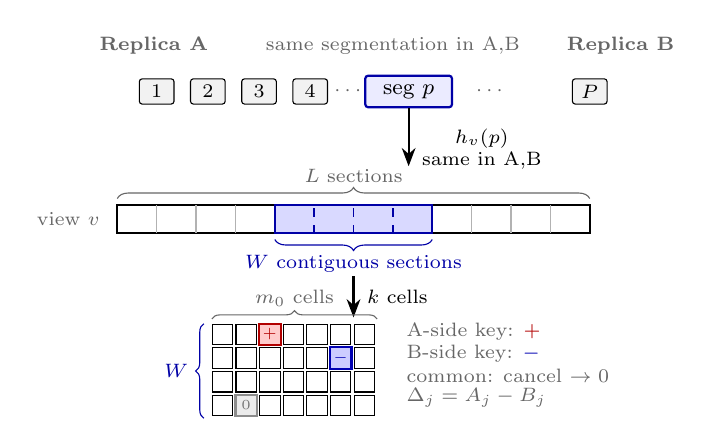
\begin{tikzpicture}[
    x=1cm, y=1cm, font=\footnotesize, >=Stealth,
    seg/.style    = {draw, rounded corners=1pt, fill=black!5,
                     inner sep=2pt, minimum height=0.40cm},
    segHi/.style  = {seg, draw=blue!65!black, line width=0.8pt, fill=blue!8},
    segSmall/.style = {draw, rounded corners=1pt, fill=black!5,
                       inner sep=0pt, minimum width=0.44cm,
                       minimum height=0.32cm, font=\scriptsize},
    cell/.style   = {draw, inner sep=0pt, minimum size=0.26cm},
    lbl/.style    = {font=\scriptsize, align=center, inner sep=1.5pt},
    note/.style   = {font=\scriptsize, text=black!60},
    arrlbl/.style = {font=\scriptsize, align=center, fill=white,
                     fill opacity=.92, text opacity=1, inner sep=1.5pt},
  ]

  % ================================================================
  % Top: segments shared by A and B
  % ================================================================
  \def\sy{0.0}

  % (4) reduce vertical gap between the "Replica ..." row and segment row
  \node[note, anchor=south west] at (0.05, \sy+0.35) {\textbf{Replica A}};
  \node[note, anchor=south east] at (7.60, \sy+0.35) {\textbf{Replica B}};
  \node[note, anchor=south]      at (3.90, \sy+0.35) {same segmentation in A,B};

  \node[segSmall] (s1) at (0.90, \sy) {1};
  \node[segSmall] (s2) at (1.55, \sy) {2};
  \node[segSmall] (s3) at (2.20, \sy) {3};
  \node[segSmall] (s4) at (2.85, \sy) {4};
  \node[note]     at (3.35, \sy) {$\cdots$};
  \node[segHi, minimum width=1.10cm] (sp) at (4.10, \sy) {seg $p$};
  \node[note]     at (5.15, \sy) {$\cdots$};
  \node[segSmall] (sP) at (6.40, \sy) {$P$};

  % (1) put "same in A,B" together with h_v(p) label
  \draw[->, thick] (sp.south) -- (4.10, -0.95)
    node[arrlbl, pos=0.7, right=3pt, align=center] {$h_v(p)$\\{\scriptsize same in A,B}};

  % ================================================================
  % Section strip with a contiguous W-window
  % ================================================================
  \def\stripX{0.40}
  \def\stripY{-1.80}
  \def\nSec{12}
  \def\cw{0.50}
  \def\stripH{0.36}
  \def\wStart{4}
  \def\Wwin{4}

  \draw[thick] (\stripX,\stripY)
    rectangle ({\stripX+\nSec*\cw},{\stripY+\stripH});
  \foreach \i in {1,...,11} {
    \draw[thin, black!30]
      ({\stripX+\i*\cw},\stripY)
      -- ({\stripX+\i*\cw},{\stripY+\stripH});
  }

  % Blue window fill + border
  \fill[blue!15]
    ({\stripX+\wStart*\cw},\stripY)
    rectangle ({\stripX+(\wStart+\Wwin)*\cw},{\stripY+\stripH});
  \draw[thick, blue!65!black]
    ({\stripX+\wStart*\cw},\stripY)
    rectangle ({\stripX+(\wStart+\Wwin)*\cw},{\stripY+\stripH});

  % W-1 dashed separators inside the window
  \foreach \t in {1,...,3} { % assumes Wwin=4
    \draw[blue!65!black, dashed, line width=0.6pt]
      ({\stripX+(\wStart+\t)*\cw},\stripY)
      -- ({\stripX+(\wStart+\t)*\cw},{\stripY+\stripH});
  }

  % (2) remove the 4 "W" letters inside the window sections
  % (removed)

  % L brace on top
  \draw[decorate, decoration={brace, amplitude=4pt}, black!60]
    ({\stripX},{\stripY+\stripH+0.08})
    -- ({\stripX+\nSec*\cw},{\stripY+\stripH+0.08})
    node[midway, above=4pt, lbl] {$L$ sections};

  % (3) change label text to "W contiguous sections"
  \draw[decorate, decoration={brace, amplitude=4pt, mirror}, blue!65!black]
    ({\stripX+\wStart*\cw},{\stripY-0.08})
    -- ({\stripX+(\wStart+\Wwin)*\cw},{\stripY-0.08})
    node[midway, below=4pt, lbl, text=blue!65!black]
    {$W$ contiguous sections};

  \node[note, anchor=east] at ({\stripX-0.10},{\stripY+\stripH/2})
    {view $v$};

  % (5) shorten the black arrow a bit (end slightly above the brace/grid top)
  \draw[->, thick]
    ({\stripX+(\wStart+\Wwin/2)*\cw}, {\stripY-0.55})
    -- ({\stripX+(\wStart+\Wwin/2)*\cw}, {\stripY-1.07})
    node[arrlbl, midway, right=3pt] {$k$ cells};

  % ================================================================
  % Window-expanded cell plane: W (rows) x m0 (cols)
  % ================================================================
  \def\gx{1.60}
  \def\gy{-2.95}
  \def\cs{0.30}
  \def\nRow{4}  % visual W
  \def\nCol{7}  % visual m0

  % Grid
  \foreach \r in {0,...,3} {
    \foreach \c in {0,...,6} {
      \node[cell, anchor=north west] (c\r\c)
        at ({\gx+\c*\cs},{\gy-\r*\cs}) {};
    }
  }

  % m0 brace (top)
  \draw[decorate, decoration={brace, amplitude=3pt}, black!60]
    ({\gx},{\gy+0.06}) -- ({\gx+\nCol*\cs},{\gy+0.06})
    node[midway, above=3pt, lbl] {$m_0$ cells};

  % W brace (left)
  \draw[decorate, decoration={brace, amplitude=3pt, mirror}, blue!65!black]
    ({\gx-0.10},{\gy})
    -- ({\gx-0.10},{\gy-\nRow*\cs})
    node[midway, left=4pt, lbl, text=blue!65!black] {$W$};

  % Example signed updates
  \fill[red!20]   (c02.north west) rectangle (c02.south east);
  \draw[thick, red!70!black] (c02.north west) rectangle (c02.south east);
  \node[font=\tiny, red!70!black] at (c02) {$+$};

  \fill[blue!20]  (c15.north west) rectangle (c15.south east);
  \draw[thick, blue!70!black] (c15.north west) rectangle (c15.south east);
  \node[font=\tiny, blue!70!black] at (c15) {$-$};

  \fill[black!8]  (c31.north west) rectangle (c31.south east);
  \draw[thick, black!45] (c31.north west) rectangle (c31.south east);
  \node[font=\tiny, black!55] at (c31) {$0$};

  % (6) tighten line spacing on the right text block
  \node[note, anchor=west, align=left]
    at ({\gx+\nCol*\cs+0.25},{\gy-0.10})
    {A-side key: \textcolor{red!70!black}{$+$}};
  \node[note, anchor=west, align=left]
    at ({\gx+\nCol*\cs+0.25},{\gy-0.38})
    {B-side key: \textcolor{blue!70!black}{$-$}};
  \node[note, anchor=west, align=left]
    at ({\gx+\nCol*\cs+0.25},{\gy-0.66})
    {common: cancel $\to 0$};
  \node[note, anchor=west, align=left]
    at ({\gx+\nCol*\cs+0.25},{\gy-0.94})
    {$\Delta_j = A_j - B_j$};

\end{tikzpicture}
\caption{Two-level mapping in one view: segment $p$ is hashed
to $W$ contiguous sections, then each key is hashed to $k$
cells within that window.}
\label{fig:scout-mapping-structure-a}
\end{figure}

%\paragraph{Pipeline}
\noindent\textbf{Pipeline}\quad
Each reconciliation cycle executes four stages; the first
three are fixed-cost, while the fourth adapts to the observed
evidence.

\textbf{(1)~Build.}  Each replica sequentially scans its local key space; every item is inserted into the probe array via the two-level mapping described above.

\textbf{(2)~Exchange \& Diff.}  The two replicas exchange
their probes once; each side subtracts cell-wise to obtain the
difference array
$\Delta_j = C^{(A)}_j - C^{(B)}_j$.
Because both replicas apply identical hash mappings to each
item, any item present on both sides produces equal updates to
the same probe cells.  These contributions cancel under
cell-wise subtraction, so $\Delta$ is driven solely by items
that differ between the two sides: items in $A\setminus B$
contribute $+1$ signed updates, while those in
$B\setminus A$ contribute~$-1$.

\textbf{(3)~Decode.}  For every section~$s$ in each view, the decoder computes the first moment and the raw second moment:
\[
\mathrm{net\_sum}_s = \sum_{j \in s}\Delta_j
,~
\mathrm{sq\_sum}_s = \sum_{j \in s}\Delta_j^2,
\]
then constructs the \textbf{de-drifted energy}:
\begin{equation*}
E_s \;=\; \mathrm{sq\_sum}_s \;-\;
         \frac{(\mathrm{net\_sum}_s)^{2}}{m_0}.
\end{equation*}
$E_s$ is the unnormalized sample variance of the differential
counts within section~$s$.  It serves as the \emph{common signal}
from which all three outputs are derived: triage consumes the
spatial distribution of $\{E_s\}$ (where energy concentrates),
sizing consumes the total mass $\sum_s E_s$ (how much energy
exists), and gating consumes the support dispersion of
$\{E_s\}$ (over how many sections energy spreads).  All three
readings come from the same energy spectrum
without budget
partitioning.  The subtraction of $(\mathrm{net\_sum}_s)^2/m_0$ removes the
first-order sign bias that would otherwise dominate the raw
second moment under side imbalance, so $E_s$ captures
fluctuation energy rather than drift-induced offset (note that
$E_s \ge 0$ by the Cauchy--Schwarz inequality). The full
derivation is given in
Supplement~\ref{sec:appendix-sizing-derivation}.

\textbf{(4)~Decide.} 
Each diagnostic output reads the same section-level energy
spectrum but fuses information across the $V$ views
differently. Sizing computes a per-view scale estimate and averages across views. 
Gating evaluates the concentration metric and occupancy on the energy spectrum (\S\ref{sec:gating}). Triage retains per-view window rankings and intersects the resulting candidate supersets to suppress view-dependent false inclusions.

When all sections in a segment's mapped window carry zero
signal ($E_s{=}0$ and $\mathrm{net\_sum}_s{=}0$) in any view, the segment can be excluded from downstream
verification, because any diff key would have left a
non-zero cell update within the window
(Supplement~\ref{sec:appendix-sizing-zero-energy}).

Sizing emits $\hat{D}$ (\S\ref{sec:dedrift});
$\hat{D}\approx 0$ terminates the round without downstream
verification.  Otherwise, gating tests $K_{\mathrm{eff}}/L$
and occupancy (\S\ref{sec:gating}).
On \texttt{notgate}, triage produces~$\mathcal{C}$ via
sliding-window aggregation and cross-view intersection
(Fig.~\ref{fig:scout-mapping-structure-b}).
On \texttt{gate}, the system suppresses candidate generation
and defers to a conservative fallback---e.g., full-scope exact
verification or a coarse per-range checksum pass over all $P$
segments---whose cost scales with $P$ rather than
$|\mathcal{C}|$.
On \texttt{unknown}, the probe withholds only a shape-based verdict; downstream policy may still invoke capped triage or full-scope fallback
based on $\hat{D}$ and other observables (\S\ref{sec:eval-dedrift}).

\begin{figure}[!htbp]
\centering
% SCOUT probe structure (b): 2 views + reverse mapping + (implicit) intersection + energy peak
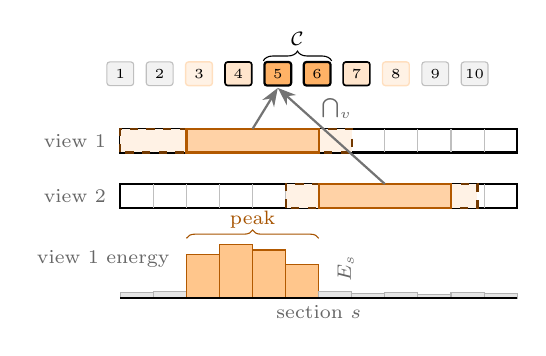
\begin{tikzpicture}[
    x=1cm, y=1cm, font=\footnotesize, >=Stealth,
    lbl/.style    = {font=\scriptsize, align=center, inner sep=1.5pt},
    note/.style   = {font=\scriptsize, text=black!60},
    arrlbl/.style = {font=\scriptsize, align=center, fill=white,
                     fill opacity=.92, text opacity=1, inner sep=1.5pt},
    segbox/.style = {draw, rounded corners=1pt, minimum width=0.34cm,
                     minimum height=0.30cm, inner sep=0pt, font=\tiny},
  ]

  % ----------------------------------------------------------------
  % Geometry knobs
  % ----------------------------------------------------------------
  \def\mvX{0.65}
  \def\mvN{12}
  \def\mvW{0.42}
  \def\mvH{0.30}
  \def\mvGap{0.70}
  \pgfmathsetmacro{\stripRight}{\mvX+\mvN*\mvW}

  % ----------------------------------------------------------------
  % Segment row (top)
  % ----------------------------------------------------------------
  \def\segX{\mvX}
  \def\segY{0.45}
  \def\segN{10}
  \def\segW{0.50}

  % segments: 1..10
  % true hot: 5,6 ; halo (normal): 4,7 ; halo (small): 3,8 ; rest: neutral
  \foreach \i in {0,...,9} {
    \pgfmathtruncatemacro{\sid}{\i+1}
    \pgfmathtruncatemacro{\isHot}{(\sid==5 || \sid==6) ? 1 : 0}
    \pgfmathtruncatemacro{\isHalo}{(\sid==4 || \sid==7) ? 1 : 0}
    \pgfmathtruncatemacro{\isHaloSmall}{(\sid==3 || \sid==8) ? 1 : 0}

    \ifnum\isHot=1
      \node[segbox, fill=orange!60, line width=0.8pt]
        (seg\sid) at ({\segX+\i*\segW},{\segY}) {\sid};
    \else
      \ifnum\isHalo=1
        \node[segbox, fill=orange!20, line width=0.6pt]
          (seg\sid) at ({\segX+\i*\segW},{\segY}) {\sid};
      \else
        \ifnum\isHaloSmall=1
          \node[segbox, fill=orange!10, draw=orange!25, line width=0.5pt]
            (seg\sid) at ({\segX+\i*\segW},{\segY}) {\sid};
        \else
          \node[segbox, fill=black!5, draw=black!25]
            (seg\sid) at ({\segX+\i*\segW},{\segY}) {\sid};
        \fi
      \fi
    \fi
  }

  % ----------------------------------------------------------------
  % Two view strips (middle)
  % ----------------------------------------------------------------
  \def\mvYstart{-0.55}

  % View 1: selected window at sections 2–5
  \pgfmathsetmacro{\yyA}{\mvYstart}
  \draw[thick] (\mvX,\yyA) rectangle (\stripRight,{\yyA+\mvH});
  \foreach \i in {1,...,11} {
    \draw[thin, black!25]
      ({\mvX+\i*\mvW},\yyA) -- ({\mvX+\i*\mvW},{\yyA+\mvH});
  }
  % halo-ish neighbors (dashed)
  \fill[orange!10]
    ({\mvX+0*\mvW},\yyA) rectangle ({\mvX+2*\mvW},{\yyA+\mvH});
  \draw[thick, orange!45!black, dashed]
    ({\mvX+0*\mvW},\yyA) rectangle ({\mvX+2*\mvW},{\yyA+\mvH});
  \fill[orange!10]
    ({\mvX+6*\mvW},\yyA) rectangle ({\mvX+7*\mvW},{\yyA+\mvH});
  \draw[thick, orange!45!black, dashed]
    ({\mvX+6*\mvW},\yyA) rectangle ({\mvX+7*\mvW},{\yyA+\mvH});
  % main selected window (solid)
  \fill[orange!35]
    ({\mvX+2*\mvW},\yyA) rectangle ({\mvX+6*\mvW},{\yyA+\mvH});
  \draw[thick, orange!70!black]
    ({\mvX+2*\mvW},\yyA) rectangle ({\mvX+6*\mvW},{\yyA+\mvH});
  \node[note, anchor=east] at ({\mvX-0.06},{\yyA+\mvH/2}) {view 1};

  % View 2: selected window at sections 6–9
  \pgfmathsetmacro{\yyB}{\mvYstart - \mvGap}
  \draw[thick] (\mvX,\yyB) rectangle (\stripRight,{\yyB+\mvH});
  \foreach \i in {1,...,11} {
    \draw[thin, black!25]
      ({\mvX+\i*\mvW},\yyB) -- ({\mvX+\i*\mvW},{\yyB+\mvH});
  }
  % halo-ish neighbors (dashed)
  \fill[orange!10]
    ({\mvX+5*\mvW},\yyB) rectangle ({\mvX+6*\mvW},{\yyB+\mvH});
  \draw[thick, orange!45!black, dashed]
    ({\mvX+5*\mvW},\yyB) rectangle ({\mvX+6*\mvW},{\yyB+\mvH});
  \fill[orange!10]
    ({\mvX+10*\mvW},\yyB) rectangle ({\mvX+10.8*\mvW},{\yyB+\mvH});
  \draw[thick, orange!45!black, dashed]
    ({\mvX+10*\mvW},\yyB) rectangle ({\mvX+10.8*\mvW},{\yyB+\mvH});
  % main selected window (solid)
  \fill[orange!35]
    ({\mvX+6*\mvW},\yyB) rectangle ({\mvX+10*\mvW},{\yyB+\mvH});
  \draw[thick, orange!70!black]
    ({\mvX+6*\mvW},\yyB) rectangle ({\mvX+10*\mvW},{\yyB+\mvH});
  \node[note, anchor=east] at ({\mvX-0.06},{\yyB+\mvH/2}) {view 2};

  % ----------------------------------------------------------------
  % Reverse-mapping arrows (avoid crossing)
  % ----------------------------------------------------------------
  % View1 arrow -> near seg5
  \coordinate (v1c) at ({\mvX+4*\mvW},{\yyA+\mvH});
  \coordinate (s1c) at ({\segX+4*\segW},{\segY-0.18}); % around seg5
  \draw[->, thick, black!55] (v1c) -- (s1c);

  % View2 arrow -> near seg5
  \coordinate (v2c) at ({\mvX+8*\mvW},{\yyB+\mvH});
  \coordinate (s2c) at ({\segX+4*\segW},{\segY-0.18}); % around seg5
  \draw[->, thick, black!55] (v2c) -- (s2c);

  % ----------------------------------------------------------------
  % Intersection marker above segment row: brace over seg5..6 labeled \mathcal{C}
  % (keep the brace, but move \bigcap_v to below seg6)
  \draw[decorate, decoration={brace, amplitude=3.5pt}]
    (seg5.north west) -- (seg6.north east)
    node[midway, above=4pt, lbl] {$\mathcal{C}$};

  % \bigcap_v moved to below seg6
  \node[note, anchor=north] at ($(seg6.south)+(0.25,-0.02)$) {$\bigcap_v$};

  % ----------------------------------------------------------------
  % Energy spectrum (bottom) — simplified labels
  % ----------------------------------------------------------------
  \pgfmathsetmacro{\barY}{\yyB - 1.15}
  \def\barX{\mvX}
  \def\barW{\mvW}
  \def\barScale{0.85}

  % Bars: peak aligned with view-1 selected window (sections 2–5)
  \foreach \idx/\ht in {
    0/0.08, 1/0.10,
    2/0.65, 3/0.80, 4/0.72, 5/0.50,
    6/0.10, 7/0.07, 8/0.09, 9/0.06, 10/0.08, 11/0.07} {
    \pgfmathsetmacro{\bh}{\ht*\barScale}
    \pgfmathtruncatemacro{\isPeak}{(\idx>=2 && \idx<=5) ? 1 : 0}
    \ifnum\isPeak=1
      \fill[orange!45]
        ({\barX+\idx*\barW},\barY)
        rectangle ({\barX+(\idx+1)*\barW},{\barY+\bh});
      \draw[orange!70!black]
        ({\barX+\idx*\barW},\barY)
        rectangle ({\barX+(\idx+1)*\barW},{\barY+\bh});
    \else
      \fill[black!10]
        ({\barX+\idx*\barW},\barY)
        rectangle ({\barX+(\idx+1)*\barW},{\barY+\bh});
      \draw[black!30]
        ({\barX+\idx*\barW},\barY)
        rectangle ({\barX+(\idx+1)*\barW},{\barY+\bh});
    \fi
  }
  \draw[thick] (\barX,\barY) -- ({\barX+12*\barW},\barY);

  % x-label
  \node[note] at ({\barX+6*\barW},{\barY-0.18}) {section $s$};

  % Move E_s to the right of the peak (avoid overlap with left label)
  \node[note, rotate=90, anchor=south]
    at ({\barX+7.35*\barW},{\barY+0.45*\barScale}) {$E_s$};

  % peak brace with only "peak"
  \draw[decorate, decoration={brace, amplitude=3pt}, orange!65!black]
    ({\barX+2*\barW},{\barY+0.80*\barScale+0.08})
    -- ({\barX+6*\barW},{\barY+0.80*\barScale+0.08})
    node[midway, above=2pt, lbl, text=orange!65!black] {peak};

  % Left label: align nicely (same x as strip labels), no overlap
  \node[note, anchor=east, align=left]
    at ({\mvX+0.75},{\barY+0.50})
    {view 1 energy};

\end{tikzpicture}
\caption{From energy peaks to candidate segments:
sliding-window aggregation identifies high-energy regions on
the section axis; reverse mapping and cross-view intersection
yield the candidate set~$\mathcal{C}$.}
\label{fig:scout-mapping-structure-b}
\end{figure}

Beyond the unavoidable single sequential scan over local items,
SCOUT incurs communication proportional to the fixed probe
size and decoding cost of $O(VLm_0)$.
Table~\ref{tab:scout-params} summarizes the core probe
parameters.

\begin{table}[!htbp]
\caption{Quick reference for SCOUT core parameters.
Full symbol table in Supplement~\ref{sec:notations}.}
\label{tab:scout-params}
\centering
\small
\setlength{\tabcolsep}{4pt}
\begin{tabular}{@{}cl@{}}
\toprule
Symbol & Meaning \\
\midrule
$P$ & Total segments ($10^4$--$10^7$) \\
$B$ & Concurrently dirty segments (unknown at runtime) \\
$D$ & Symmetric difference size, $D=D^{+}+D^{-}$ \\
$V$ & Views / independent hash channels (2--4) \\
$L$ & Sections per view (1024--8192) \\
$m_0$ & Cells per section (16--64) \\
$W$ & Window width in contiguous sections (2--4) \\
$k$ & Per-key update redundancy (1--3) \\
\bottomrule
\end{tabular}
\end{table}


\subsection{Observation Geometry for Candidate Compression}
\label{sec:spatial-coupling}

Triage operates on the energy spectrum $\{E_s\}$.
Its ability to compress the candidate set depends on whether
dirty-segment energy remains localized on the section axis.
Localized energy produces separable peaks and enables
candidate compression; dispersed energy blends into
background noise and reduces triage to broad ranking.


\paragraph{Contiguous-interval mapping and sliding-window aggregation}
To preserve locality, SCOUT maps each segment to $W$
\textbf{contiguous} sections on the section axis.  Triage
therefore scores \emph{windows} rather than individual
sections.  For each starting position~$u$, SCOUT computes
\[
\Omega_u = \sum_{s=u}^{u+W-1} E_s,
\]
the total energy in the width-$W$ window beginning at~$u$.
This sliding-window aggregation pools the energy that a single
segment deposits across its $W$ adjacent sections, strengthening
localized peaks while suppressing unstructured background
noise---a width-$W$ matched filter in signal-processing terms.

SCOUT then ranks all windows by~$\Omega_u$ and keeps the top
$
t = \left\lceil r_{\mathrm{top}} \cdot (L-W+1) \right\rceil
$
windows, where $r_{\mathrm{top}} \in (0,1]$ controls the
candidate budget. Each selected window is then reverse-mapped
to the segments whose supports overlap it
(Fig.~\ref{fig:scout-mapping-structure-b}), producing a
view-local candidate superset.
The final candidate set~$\mathcal{C}$ is obtained by
intersecting these supersets across all $V$ views, which
suppresses false inclusions exponentially under approximately
independent views while preserving true positives with high
probability.

The compression effect above depends on \emph{contiguity}: if
the $W$ target sections were scattered randomly instead of
placed contiguously, the sliding window would lose its locality
advantage and the scheme would reduce to independent
per-section ranking (\S\ref{sec:eval-spatial}).

\paragraph{Scaling laws for candidate-set size}
Under the uniform-hashing model (\S\ref{sec:overview}),
if concentrated differences produce separable signals,
the expected candidate-set size after intersecting across $V$
views is:
\begin{equation}\label{eq:cand-expectation}
\mathbb{E}[|\mathcal{C}|]
  \;\approx\; B \;+\; (P-B)\cdot p_{\mathrm{halo}}^{\,V},
\end{equation}
where $B$ is the number of truly dirty segments and the second
term captures the \emph{halo} contribution: clean segments whose
windows geometrically overlap with a selected dirty window are
erroneously included in the candidate set.
A clean segment's false-inclusion probability in a single view
is
\begin{equation}\label{eq:halo-prob}
p_{\mathrm{halo}}
  \;\approx\; \frac{t(2W-1)}{L}
  \quad(\text{when } t(2W-1) \ll L),
\end{equation}
where $2W{-}1$ is the overlap neighborhood width of each
selected window on the section axis.
This framework implies three scaling laws:
(i)~cross-view intersection raises $p_{\mathrm{halo}}$ to the
$V$-th power, making $V$ the most effective lever against
candidate inflation;
(ii) the halo term grows with the number of clean segments,
while larger $L$ reduces per-view overlap and suppresses false
inclusion;
(iii)~$W$ improves signal aggregation but simultaneously
inflates the halo via the $2W{-}1$ factor, so there is no
uniformly optimal~$W$
(derivations in Supplement~\ref{sec:appendix-candidate-expectation}
and~\ref{sec:appendix-w-pricing}).
All three laws require that dirty windows remain separable
on the section axis; when $L/B$ is too small, their supports
overlap and candidate cost degrades sharply.
This operating boundary is characterized empirically in
\S\ref{sec:eval-operating} and modeled in
Supplement~\ref{sec:appendix-operating-theory}.


\subsection{Drift-Stable Sizing from the Shared Substrate}
\label{sec:dedrift}

The de-drifted energy~$E_s$ (\S\ref{sec:overview}) removes
the first-order sign bias that would otherwise cause sizing
to overestimate by orders of magnitude under drift; we now
derive the estimator built on it.
Let $M = L \cdot m_0$ denote the total cell count
of a single view.
Under the same uniform-hashing model, the expected total
de-drifted energy is:
\[
\mathbb{E}\!\left[\sum_s E_s\right]
  \;=\; D \cdot k\!\left(1 - \frac{k}{M}\right).
\]
Mean subtraction cancels the drift factor~$(2q{-}1)^2$
exactly: both the squared-mean component of~$\mathrm{sq\_sum}$
and the correction term~$\mathrm{net\_sum}^{2}/m_0$ scale
quadratically with the mean sign bias~$(2q{-}1)$, and their
coefficients match, so after subtraction the expectation does
not depend on~$q$.
The sizing estimator is
\[
  \hat{D} \;=\; \frac{\sum_s E_s}{\,k\bigl(1 - k/M\bigr)\,},
\]
where the denominator $1{-}k/M$ corrects for energy dilution
from cross-key collisions within the same cell.

Two minor bias sources remain.
First, $E_s$ as a sample variance exhibits finite-sample
shrinkage, removable by a Bessel correction factor
$m_0/(m_0{-}1)$.
Second, when differences are highly concentrated in a few
sections the global uniformity approximation introduces a
systematic underestimate of roughly $1$--$2\%$.
After both corrections the measured relative bias converges to
within approximately $3\%$ across all tested configurations (\S\ref{sec:eval-dedrift}).

Multi-view fusion provides additional robustness:
averaging across approximately independent views drives
the standard deviation down as $1/\sqrt{V}$, making $V$
and $m_0$ the two main tuning knobs for sizing precision.
Derivations covering drift cancellation, bias
corrections, and multi-view fusion are given in
Supplement~\ref{sec:appendix-sizing-derivation}
and~\ref{sec:appendix-sizing-bias}.


\subsection{Admission and Abstention: When Not to Triage}
\label{sec:gating}

The gating decision rests on two observable quantities
derived from the energy spectrum: how broadly the energy is
spread, and whether the sketch carries enough statistical
support to make that measurement reliable.

\paragraph{Concentration metric}
We measure energy dispersion by the inverse Herfindahl index
\begin{equation*}
\frac{K_{\mathrm{eff}}}{L}
  \;=\; \frac{1}{L}\,\frac{\bigl(\sum_s E_s\bigr)^{2}}
        {\sum_s E_s^{2}}
  \;\in\; [1/L,\,1].
\end{equation*}
$K_{\mathrm{eff}}/L$ measures how many sections carry appreciable energy. It is invariant to overall discrepancy scale and to drift when computed from de-drifted energy. Under concentrated
faults, energy resides in roughly $BW$ sections, placing $K_{\mathrm{eff}}/L$ at the scale of $BW/L$, typically far below~$1$; under diffuse differences with sufficient occupancy it
approaches~$1$. In the concentrated regime, $K_{\mathrm{eff}}/L$ also governs candidate inflation: a larger value requires a more generous truncation budget to preserve recall, widening
halo overlap so that candidate cost grows as $p_{\mathrm{halo}}^V$. $K_{\mathrm{eff}}/L$ therefore serves not only as a shape statistic but as a cost-oriented proxy for whether triage
remains economical. Because concentrated and diffuse discrepancies are separated by roughly an order of magnitude in this metric, $\tau_{\text{gating}}$ needs only to fall between the two
regimes rather than be tuned precisely (derivation in Supplement~\ref{sec:appendix-gating-separation}; empirical sensitivity in \S\ref{sec:eval-dedrift}).

\paragraph{Observability guard-rail and three-state output}
The scale separation above requires sufficient statistical
support in the energy spectrum. When occupancy is low,
diffuse cases can collapse to support sizes comparable to
concentrated ones, making $K_{\mathrm{eff}}/L$ unreliable.
We define occupancy as the cross-view fraction of non-empty
sections:
\begin{equation}\label{eq:occupancy}
\mathrm{occ}
  \;=\; \frac{1}{V}\sum_{v=1}^{V}\;
        \frac{1}{L}\sum_{s=1}^{L}
        \mathbf{1}\!\bigl[E_s^{(v)} > 0\bigr],
\end{equation}
where $E_s^{(v)}$ denotes $E_s$ evaluated on view~$v$.
SCOUT uses a three-state gating rule:
$g=\texttt{unknown}$ if $\mathrm{occ}<\tau_{\mathrm{occ}}$;
otherwise, $g=\texttt{notgate}$ if $K_{\mathrm{eff}}/L\le\tau_{\mathrm{gating}}$,
and $g=\texttt{gate}$ otherwise.
Neither threshold requires narrow tuning.
$\tau_{\text{gating}}$ only needs to fall between the
concentrated and diffuse regimes of $K_{\mathrm{eff}}/L$,
a gap that remains wide whenever occupancy is sufficient
(\S\ref{sec:eval-dedrift}).
$\tau_{\text{occ}}$ only needs to exceed the typical
concentrated-fault occupancy~$BW/L$ by a moderate margin
to preserve scale separation within the observable region.

\section{Evaluation}
\label{sec:evaluation}

\subsection{Setup, Baselines, and Metrics}
\label{sec:eval-method}

The evaluation asks whether SCOUT can make reliable decisions across the discrepancy patterns that arise in continuous heterogeneous validation, without depending on any particular
engine pair. We therefore organize the evaluation around concentrated faults, diffuse discrepancies, side imbalance (drift), and increasing discrepancy scale, rather than around a specific
cross-engine deployment.

The evaluation proceeds in two stages.
Parameterized synthetic workloads
(\S\ref{sec:eval-spatial}--\S\ref{sec:eval-operating})
isolate individual mechanisms and map operating boundaries.
YCSB Zipfian workloads (\S\ref{sec:eval-ycsb}) introduce
segment-size skew and hotness imbalance to test robustness
under more realistic data-distribution conditions.
Synthetic workloads cover concentrated, diffuse, and mixed
heavy-tail patterns with explicit sweeps over drift
intensity; exact constructions are given in
Supplement~\ref{sec:appendix-workloads}.

\paragraph{Baselines}
We compare three methods under the single-round fixed-budget
constraint.
B1 (per-segment checksum) maintains one checksum per segment;
because its digest grows with~$P$, it violates the
fixed-budget constraint and serves only as a full-information
reference rather than a same-budget baseline.
B2 (CountSketch ranking) treats each segment as an item and
outputs a top-$K$ candidate set ranked by difference intensity.
B3 (hierarchical bucket tree) maps segments to leaf nodes of a
fixed-depth tree and drills down from root to leaves by selecting
high-score buckets at each level; when a leaf bucket is selected,
all segments it contains become candidates, producing step-wise
cost jumps of $P/b^d$ per bucket
(Supplement~Fig.~\ref{fig:b3_bucket_tree}). B2 and B3 represent the two most natural fixed-budget single-round alternatives in this setting: unstructured ranking and structured hierarchical aggregation.
All methods are aligned by digest memory in bytes at a primary
tier of ${\sim}512$\,KiB; each baseline is additionally tested
at ${\sim}2{\times}$ memory
(exact configurations in Supplement~Table~\ref{tab:c5-0}).

\paragraph{Metrics and operating-point selection}
The primary triage metric is the candidate fraction
$\mathtt{cand\_frac}{=}|\mathcal{C}|/P$.
For triage comparisons, we sweep each method's internal tuning
knob and report the best operating point that satisfies the
target heavy-segment recall for the experiment, where
$\mathtt{recall\_big}$ measures recall over the truly heavily
dirty segments in the workload instance. Where a candidate-budget
cap is imposed, infeasible points are marked as \textbf{N/A}.

Gating quality is evaluated through false-alarm rate (FAR) and false-rejection rate (FRR) trade-offs. When
the experiment includes abstention, we additionally report
performance on decisive (non-\texttt{unknown}) samples.
Sizing accuracy is reported as $\mathrm{Std(rel\_err)}$, the
standard deviation of the relative estimation error
$(\hat{D}-D)/D$ across repetitions.

YCSB validation scales to ${\sim}2{\times}10^9$ records across
$P{=}100{,}000$ segments with one-sided digest below 1\,MiB. Details are in
Supplement~\ref{sec:appendix-scale}.

\subsection{Spatial Coupling Enables Candidate Compression}
\label{sec:eval-spatial}

This section validates the necessity of two key design choices in spatial coupling---window support ($W>1$) and contiguous structure---for candidate compression.

\paragraph{Choice of window width}
Spatial coupling through overlapping windows ($W \ge 2$) improves ranking
quality over per-section independent scoring ($W{=}1$), but the benefit
saturates and eventually reverses as $W$ grows. The underlying trade-off
is that a wider window reduces the number of top-ranked slots needed to
cover all dirty segments, yet simultaneously expands each slot's halo
neighborhood by a factor of $2W{-}1$; a net benefit requires the ranking
compression to outpace this geometric penalty. In our ablation, $W{=}2$
matches or improves upon $W{=}1$ in all tested configurations, with
larger gains under higher collision pressure---up to $\sim$3.8$\times$
candidate cost reduction. Beyond $W{=}2$, the compression headroom is
exhausted and halo expansion dominates when $L/B$ is tight (full ablation
in Supplement~\ref{sec:appendix-w-ablation}).


\paragraph{Contiguous vs.\ random grouping}
To isolate the contribution of contiguity, we compare two
mapping topologies at $W{=}4$: \emph{contiguous windows},
where each segment maps to $W$ adjacent sections starting
from a single hashed position, and \emph{random grouping},
where the $W$ sections are chosen independently and need not
be adjacent. The two share identical physical budget and
coverage; they differ only in spatial arrangement.
Complementary evidence from the energy-coverage view is
reported in Supplement Figure~\ref{fig:c1-5}.
The diff-capture curves in Figure~\ref{fig:c1-4} show that
contiguous windows yield a markedly steeper curve: 
contiguous mapping concentrates the energy of dirty segments
into localized peaks that are amplified by sliding-window
aggregation, whereas random grouping disperses that energy
and reduces separability under collision noise.
This aligns with the
matched-filter intuition from \S\ref{sec:spatial-coupling}:
random grouping breaks the coherent alignment of the
contiguous support, eliminating the superposition gain of
window aggregation.

\begin{figure}[!htbp]
\centering
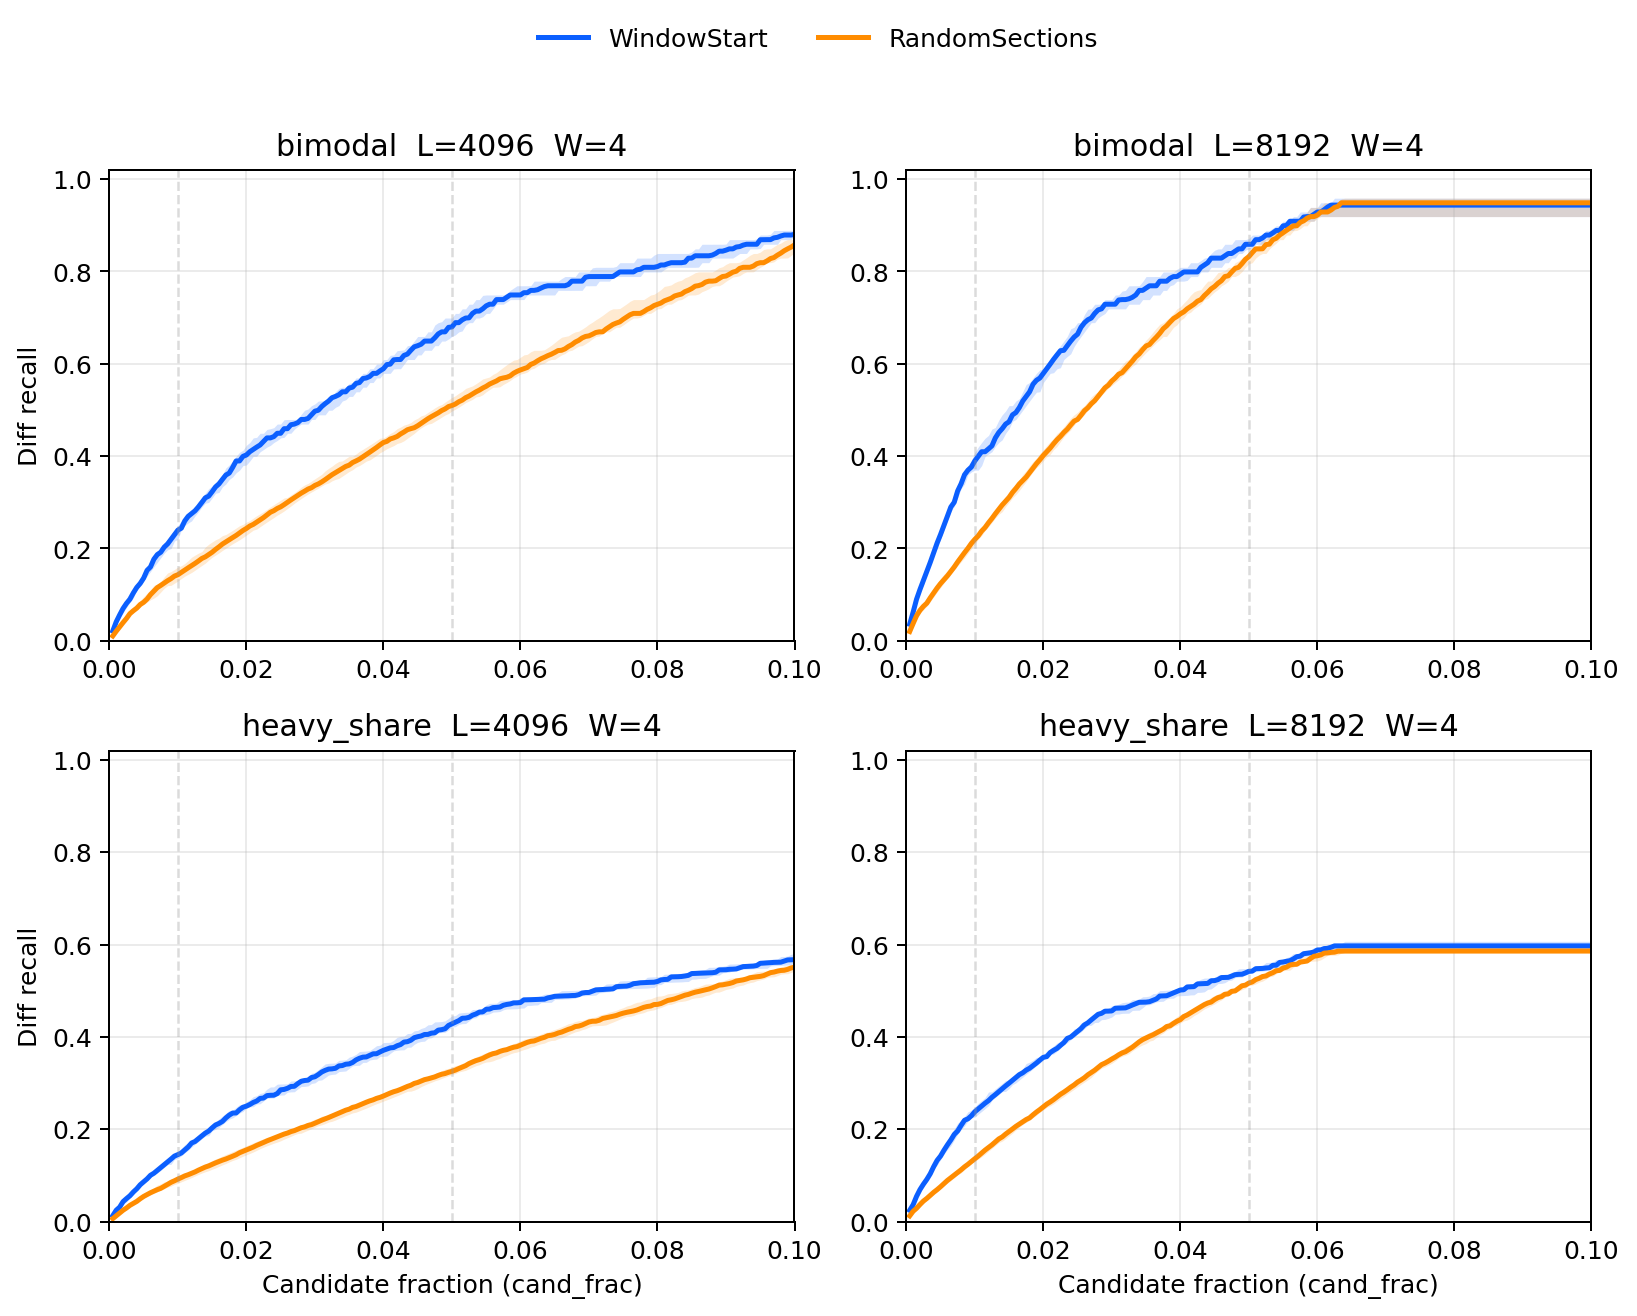
\includegraphics[width=0.95\linewidth]{figures/fig_topk_projected_window_coverage.png}
\caption{Diff capture curve: contiguous windows (\texttt{WindowStart}) vs.\ random grouping (\texttt{RandomSections}), $W{=}4$. 
Vertical axis: cumulative captured diff fraction. \texttt{bimodal} denotes concentrated pattern; \texttt{heavy\_share} denotes mixed pattern.}
\label{fig:c1-4}
\end{figure}

The trends from both experiments are consistent with the
scaling analysis in \S\ref{sec:spatial-coupling},
Equations~\eqref{eq:cand-expectation}--\eqref{eq:halo-prob},
although that analysis assumes sufficient signal separability.
When mixed or heavy-tail noise compresses the ranking margin,
the truncation quota needed to preserve recall increases, and
candidate cost rises accordingly; we characterize this
interaction further in \S\ref{sec:eval-operating}. Overall,
these results show that effective candidate compression depends
on both multi-section support ($W>1$) and contiguity, with the
main gain coming from coherent aggregation rather than simply
from increasing the number of sections touched by each segment.

\subsection{De-drift Stabilizes Sizing and Gating}
\label{sec:eval-dedrift}

We first verify drift-invariance of the de-drifted statistic, then evaluate the scaling of sizing accuracy and the reliability region of three-state gating.

\paragraph{Stability under drift}
We sweep $q$ over ${0.2, 0.5, 0.9}$ and compare the
de-drifted energy against two controls: \texttt{raw\_sq\_sum}
($\sum_j \Delta_j^2$, raw second moment, no mean removal) and
\texttt{abs\_net\_sum} ($|\sum_j \Delta_j|$, first-order absolute moment).
Table~\ref{tab:c2-unified} reports all three statistics without bias correction.

For sizing, \texttt{raw\_sq\_sum} produces overestimation above
$10^4\%$ under strong drift (Table~\ref{tab:c2-unified}),
whereas de-drifted energy keeps the error within about 10\%;
with Bessel correction this narrows further to about 3\%
(Table~\ref{tab:c3-anchor}; Supplement~Table~\ref{tab:c2-3}).

For gating, $K_{\mathrm{eff}}/L$ computed from de-drifted energy
remains nearly invariant across drift levels
(${\sim}0.015$--$0.017$). In contrast, \texttt{abs\_net\_sum} gives similarly low values under
asymmetric drift ($q \neq 0.5$) but jumps to $0.425$ at $q{=}0.5$
(Table~\ref{tab:c2-unified}). At that point the concentrated
fault is misread as diffuse (cross-configuration robustness
in Supplement~\ref{sec:appendix-dedrift}).

\begin{table}[!thbp]
\caption{Sizing and gating stability under drift. Top: sizing \texttt{rel\_err}; bottom: gating $K_{\mathrm{eff}}/L$ (\texttt{heavy\_share}).}
\label{tab:c2-unified}
\centering
\small
\setlength{\tabcolsep}{3pt}

\begin{tabular}{@{}lclrr@{}}
\toprule
\textbf{Sizing (\texttt{rel\_err})} & $q$ & workload & median & p90 \\
\midrule
\texttt{raw\_sq\_sum}        & 0.2 & bimodal & \textbf{+16\,659\%} & \textbf{17\,418\%} \\
\texttt{raw\_sq\_sum}        & 0.9 & bimodal & \textbf{+29\,576\%} & \textbf{31\,180\%} \\
\texttt{dedrift\_countscore} & 0.2 & bimodal & $-$9.1\%   & -4.1\% \\
\texttt{dedrift\_countscore} & 0.9 & bimodal & $-$8.9\%   & -3.7\% \\
\midrule
\textbf{Gating} ($K_{\mathrm{eff}}/L$) & $q$ & & \multicolumn{2}{c}{$K_{\mathrm{eff}}/L$} \\
\midrule
\texttt{dedrift\_countscore} & 0.2 & & \multicolumn{2}{c}{0.0153} \\
\texttt{dedrift\_countscore} & 0.5 & & \multicolumn{2}{c}{0.0166} \\
\texttt{dedrift\_countscore} & 0.9 & & \multicolumn{2}{c}{0.0162} \\
\texttt{abs\_net\_sum}       & 0.5 & & \multicolumn{2}{c}{\textbf{0.425}} \\
\bottomrule
\end{tabular}
\end{table}

\paragraph{Predictable scaling of sizing accuracy}
%\noindent\textbf{Predictable scaling of sizing accuracy} \quad
Multi-view fusion reduces $\mathrm{Std(rel\_err)}$ approximately as $V^{-0.5}$, consistent with the expected variance reduction from averaging near-independent views. A log-log regression across configurations yields a mean slope of $-0.498$ (std $0.050$), confirming this $V^{-0.5}$ scaling.
Increasing $m_0$ also reduces variance, as shown in Table~\ref{tab:c3-anchor}.

Moreover, $\mathrm{Std(rel\_err)}$ is weakly dependent on the discrepancy size~$D$: as it spans from $10^2$ to
$10^7$, the standard deviation remains in the approximately 2\%--3\% range, indicating that accuracy is governed primarily by probe capacity parameters rather than discrepancy magnitude (theoretical analysis, full curves, and stability verification in Supplement~\ref{sec:appendix-sizing-supp}).

\begin{table}[!htbp]
\caption{Representative configurations for sizing accuracy ($L{=}2048$). Top: fixing $m_0{=}32$ and sweeping $V$; bottom: fixing $V{=}4$ and sweeping $m_0$.}
\label{tab:c3-anchor}
\centering
\footnotesize
\begin{tabular}{lccc}
\toprule
Setting & Knob & Values & \texttt{Std(rel\_err)} (\%) \\
\midrule
\shortstack[l]{$m_0{=}32$} & $V$ & 1 / 4 / 16 & 3.53 / 2.25 / 1.01 \\
\shortstack[l]{$V{=}4$} & $m_0$ & 8 / 32 / 128 & 3.81 / 2.25 / 1.04 \\
\bottomrule
\end{tabular}
\end{table}

\paragraph{Three-state gating classification}
%\noindent\textbf{Three-state gating classification} \quad
The scale separation between concentrated and diffuse regimes
predicted in \S\ref{sec:gating} requires sufficient occupancy;
we now evaluate the practical reliability region of this
separation using the FAR--FRR trade-off over all samples
(including \texttt{unknown}).



Figure~\ref{fig:dedrift-far-frr-all} shows the unconditional
FAR--FRR Pareto front: each curve corresponds to a fixed
$\tau_{\text{occ}}$, and moving along a curve sweeps
$\tau_{\text{gating}}$.
Higher $\tau_{\text{occ}}$ generally yields lower FAR but
higher FRR. Raising the occupancy threshold excludes
ambiguous samples, improving discrimination among the
remainder and thus lowering FAR. However, because excluded
samples are counted as \texttt{unknown} rejections in the
unconditional metric, FRR rises accordingly.

Beyond $\tau_{\text{occ}} \approx 0.10$, the FRR floor settles
near 13\%. Two factors contribute: some genuinely diffuse
samples have occupancy below the threshold and are therefore
excluded as \texttt{unknown}; meanwhile, at large~$B$
(e.g., $B{=}200$, $L{=}2048$), the concentrated and diffuse
regimes converge in $K_{\text{eff}}/L$, making them
difficult to distinguish regardless of the threshold choice.

\begin{figure}[!htbp]
\centering
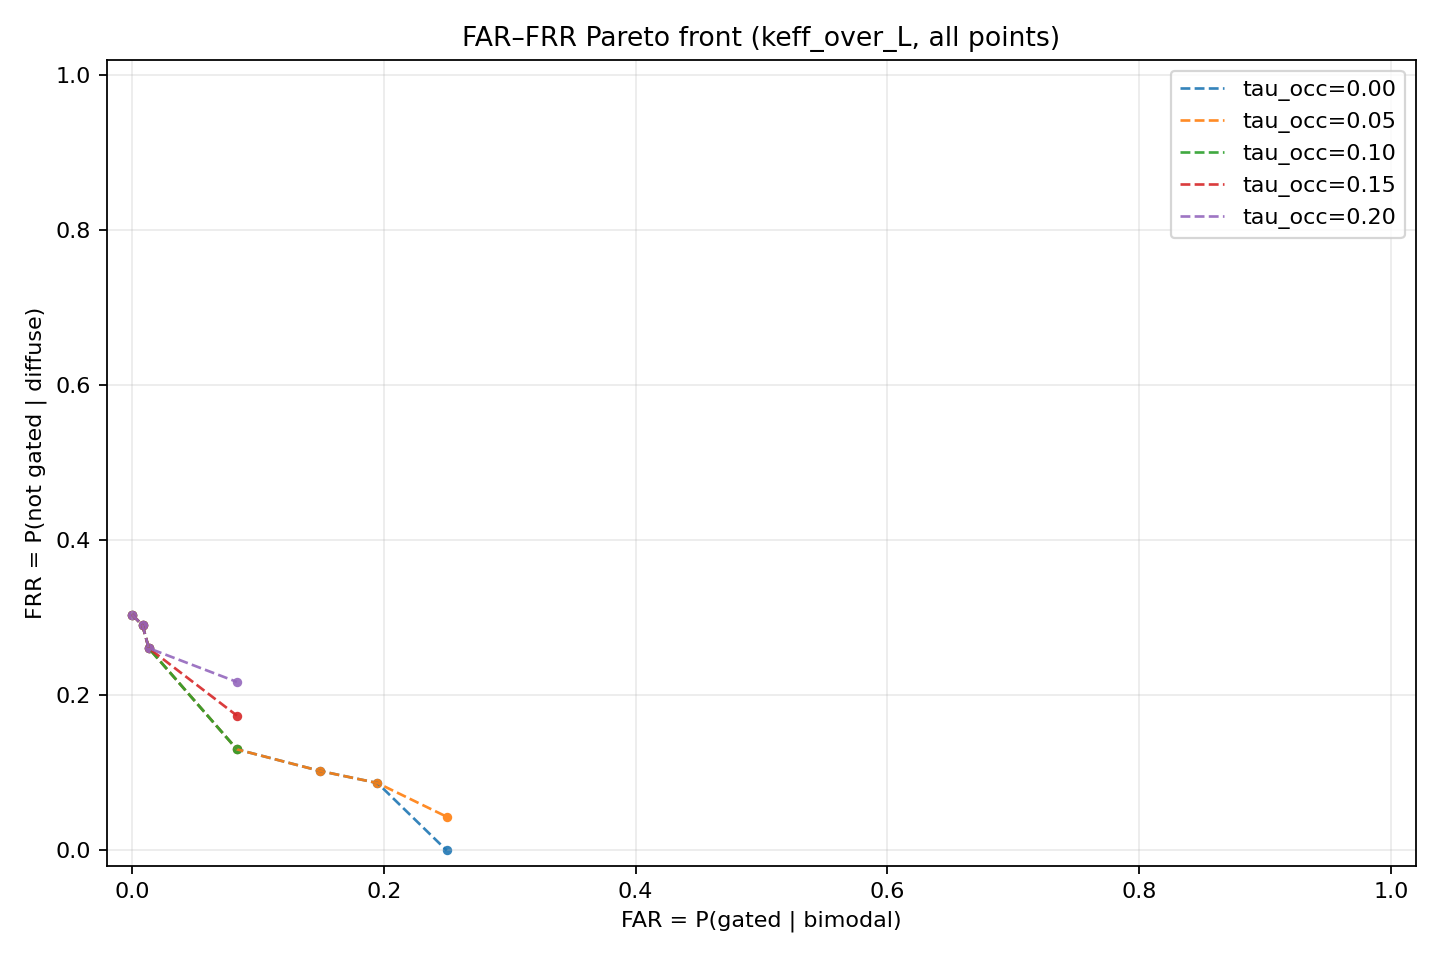
\includegraphics[width=0.95\linewidth]{figures/fig_far_frr_all_pareto.png}
\caption{Unconditional FAR--FRR trade-off. Each curve corresponds to a fixed $\tau_{\text{occ}}$; only non-dominated points are retained. Higher $\tau_{\text{occ}}$ generally yields lower FAR but higher FRR.}
\label{fig:dedrift-far-frr-all}
\end{figure}

The preceding analysis counts all samples---including those
labeled \texttt{unknown}---toward the error rates. An
alternative view considers only samples that receive a
decisive verdict (\texttt{notgate} or \texttt{gate}) and
computes \emph{conditional} error rates
$\mathrm{FAR_{cond}}$ and $\mathrm{FRR_{cond}}$ on this
subset. Under this metric, both rates can approach 0
simultaneously (Supplement Fig.~\ref{fig:dedrift-far-frr-cond}).
At $\tau_{\text{occ}}{=}0.10$, approximately 87\% of diffuse
samples still receive a decisive classification, while most
bimodal samples with small~$B$ are labeled \texttt{unknown}
due to low occupancy.
A two-state classifier would be forced to emit a verdict on
these low-support samples despite collapsed scale separation,
whereas the three-state design abstains and keeps
$\mathrm{FAR_{cond}}$ and $\mathrm{FRR_{cond}}$ near zero
among decisive verdicts.

\subsection{Operating Limits and Runtime Stopping Rule}
\label{sec:eval-operating}


\begin{figure*}[!thbp]
\centering
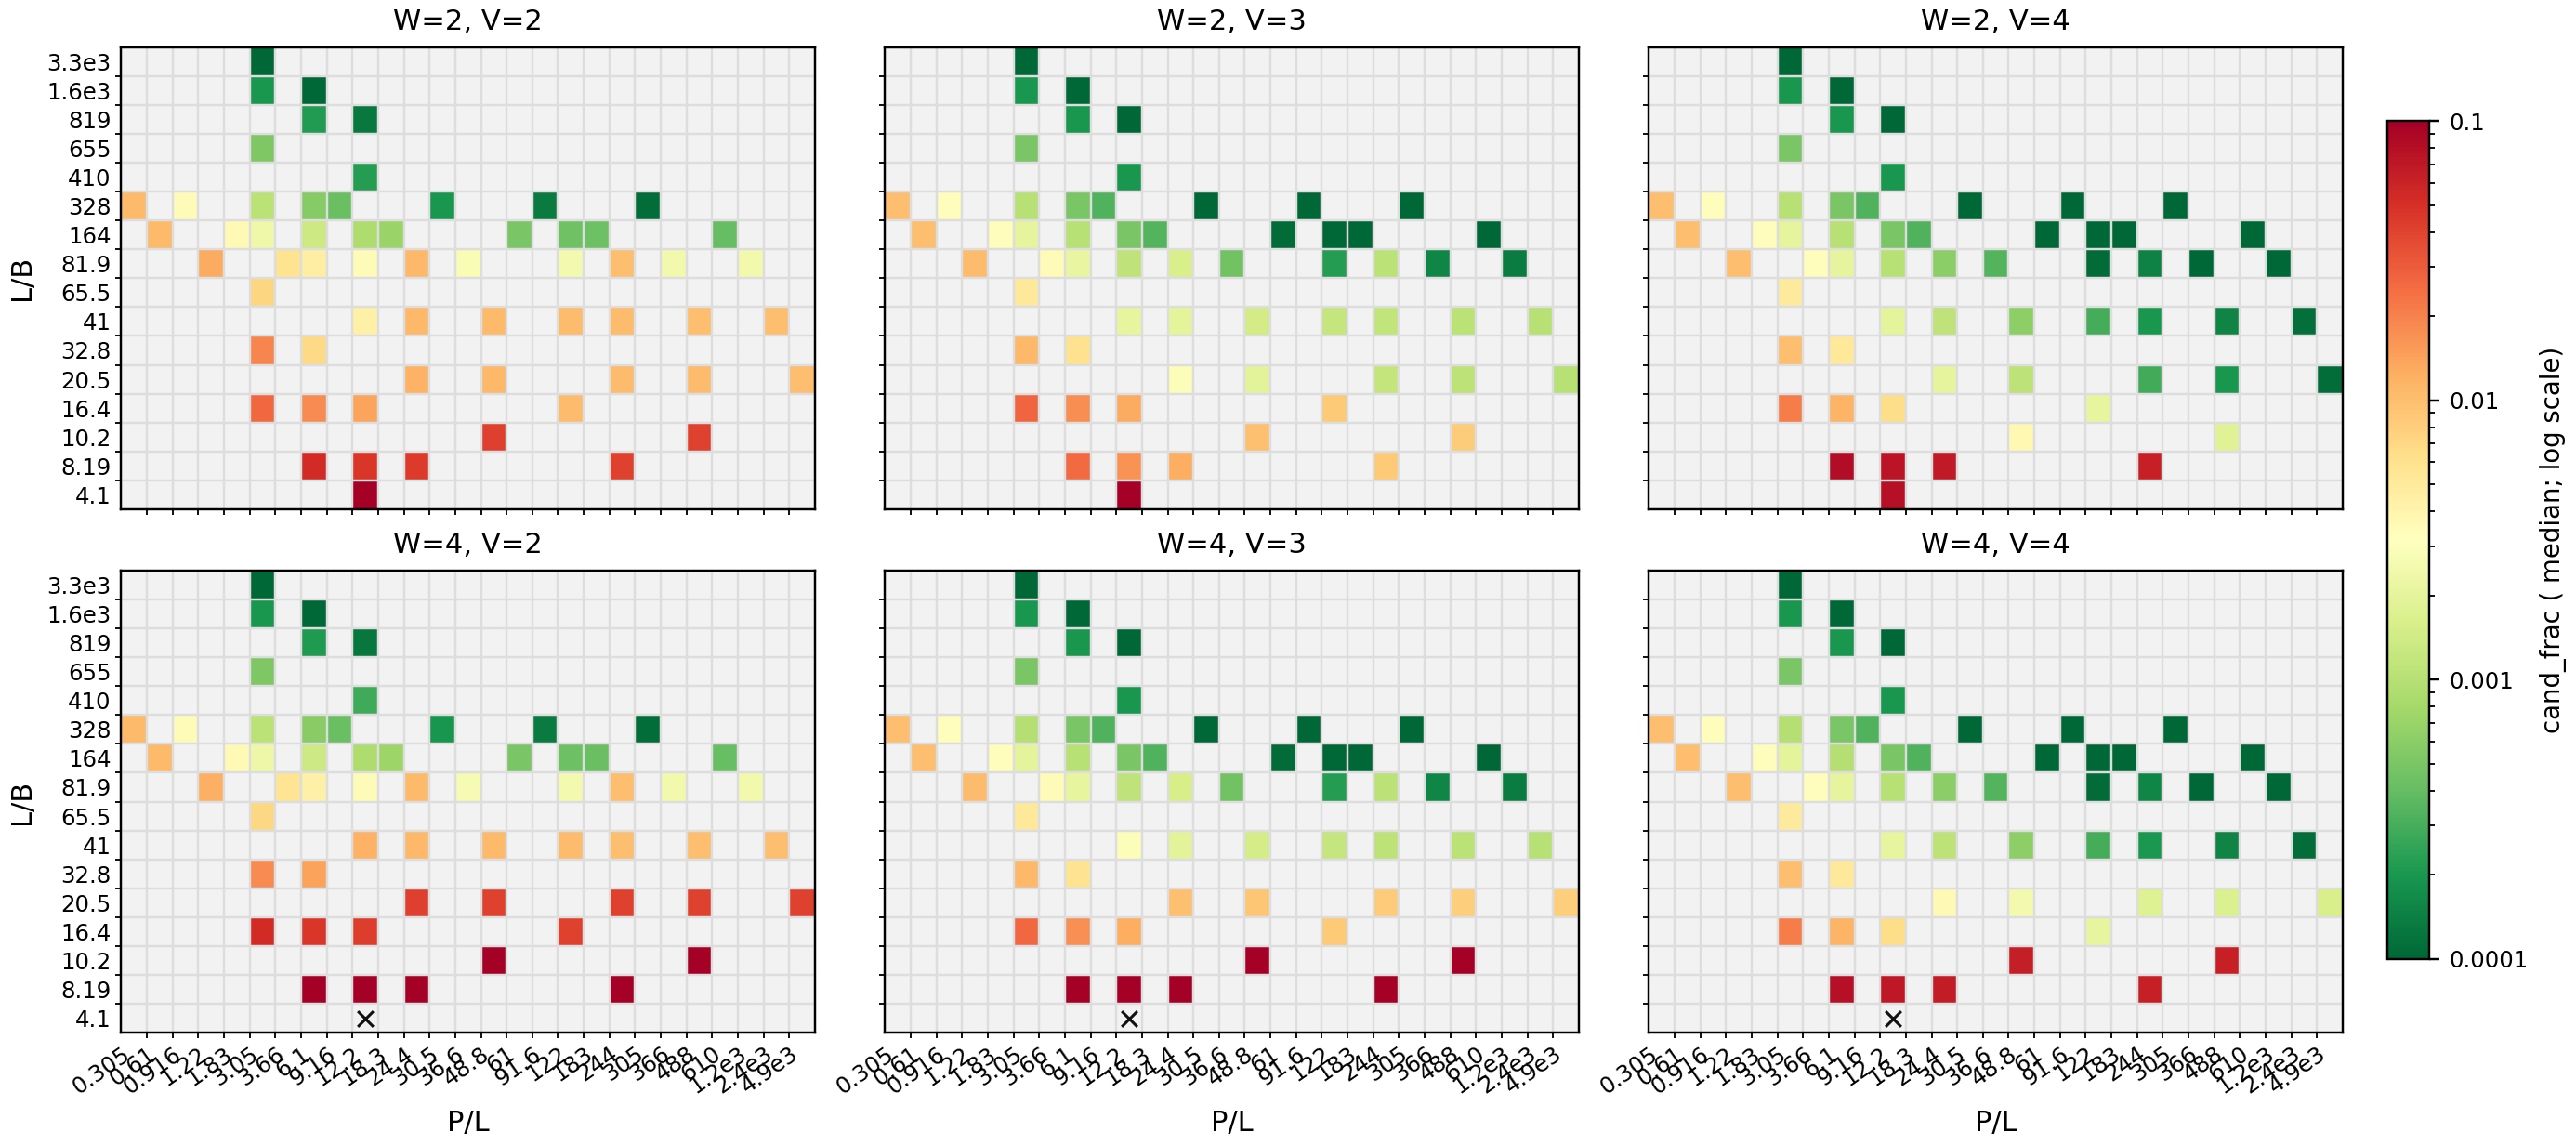
\includegraphics[width=0.93\textwidth]{figures/fig_operating_region_map_merged_heatmap.png}
 \caption{Operating region heatmap over $P/L$ and $L/B$. Color encodes the median candidate fraction \texttt{cand\_frac} on a log scale; $\times$ marks infeasible points, and gray denotes configurations with no samples.}\label{fig:c4-1}
\end{figure*}

Figure~\ref{fig:c4-1} visualizes the system's transition from effective
operation to degradation in the $(P/L,\;L/B)$ plane. The two axes govern
candidate cost through distinct mechanisms.

Along decreasing $L/B$, the $B$ dirty segments become denser on the section
axis and their high-energy windows begin to overlap, so triage must retain
more top-ranked windows to maintain recall—raising candidate cost.
Equivalently, $\texttt{cand\_frac}$ decreases monotonically with increasing
$L/B$ across all configurations. This trend is visible in the per-slice
curves of Supplement Figure~\ref{fig:c4-2}, which fix $P/L$ and sweep $L/B$.

As $P/L$ increases, the larger clean-segment pool amplifies false inclusion through the $(P-B)\,p_{\mathrm{halo}}^V$ term. 
This effect is visible even in a representative boundary slice: 
as $P/L$ grows from 1.2 to 1221,
candidate counts rise from the hundreds to the tens of thousands.
Raising $V$ from 2 to 4 reduces the count back to the hundreds,
confirming that the $P/L$-driven amplification is suppressible by
multi-view intersection (numerical details in Supplement
Table~\ref{tab:c4-1}).

Under a fixed memory budget $M_{\text{bytes}}=4VLm_0$, adding views forces $L$ to shrink proportionally ($L\propto 1/V$). More views strengthen cross-view intersection suppression exponentially, but the smaller $L$ raises the per-view halo probability $p_{\mathrm{halo}}\approx t(2W{-}1)/L$, where $t\approx \alpha BW$ and $\alpha=O(1)$ is a truncation factor. This creates a fundamental trade-off:
once $L/B$ drops below a threshold, $p_{\mathrm{halo}}$ approaches 1,
cross-view intersection loses its filtering power, and candidate cost rises
sharply. A closed-form analysis (Supplement~\ref{sec:appendix-operating-theory})
yields a sufficient condition for the intersection mechanism to remain
effective:
$
L/B \;\gtrsim\; e\alpha W(2W{-}1),
$
which evaluates to $L/B\approx 16$ for $W{=}2$, $\alpha{=}1$---the 
order of magnitude for the transition band visible in
Figure~\ref{fig:c4-1}. Above this region, the $P/L$-driven amplification
can be absorbed exponentially by multi-view intersection, and degradation
along that axis is considerably milder.


\paragraph{Runtime stopping rule}
\label{sec:eval-stoploss}
In \S\ref{sec:spatial-coupling}, triage ranks windows by energy and selects the top $t = \lceil \mathrm{r_{top}} \cdot (L-W+1) \rceil$; larger $\mathrm{r_{top}}$ yields a larger candidate set. Since $B$ is unknown at runtime and may exceed the planning prior $B^*$, SCOUT applies a runtime truncation rule.
A purely observable signal provides this adaptation. As $\mathrm{r_{top}}$ is swept upward during local decoding (a negligible in-memory computation once the probe is built), the system tracks how much energy the selected sections capture and how many candidate segments they produce.

\begin{figure}[!thbp]
\centering
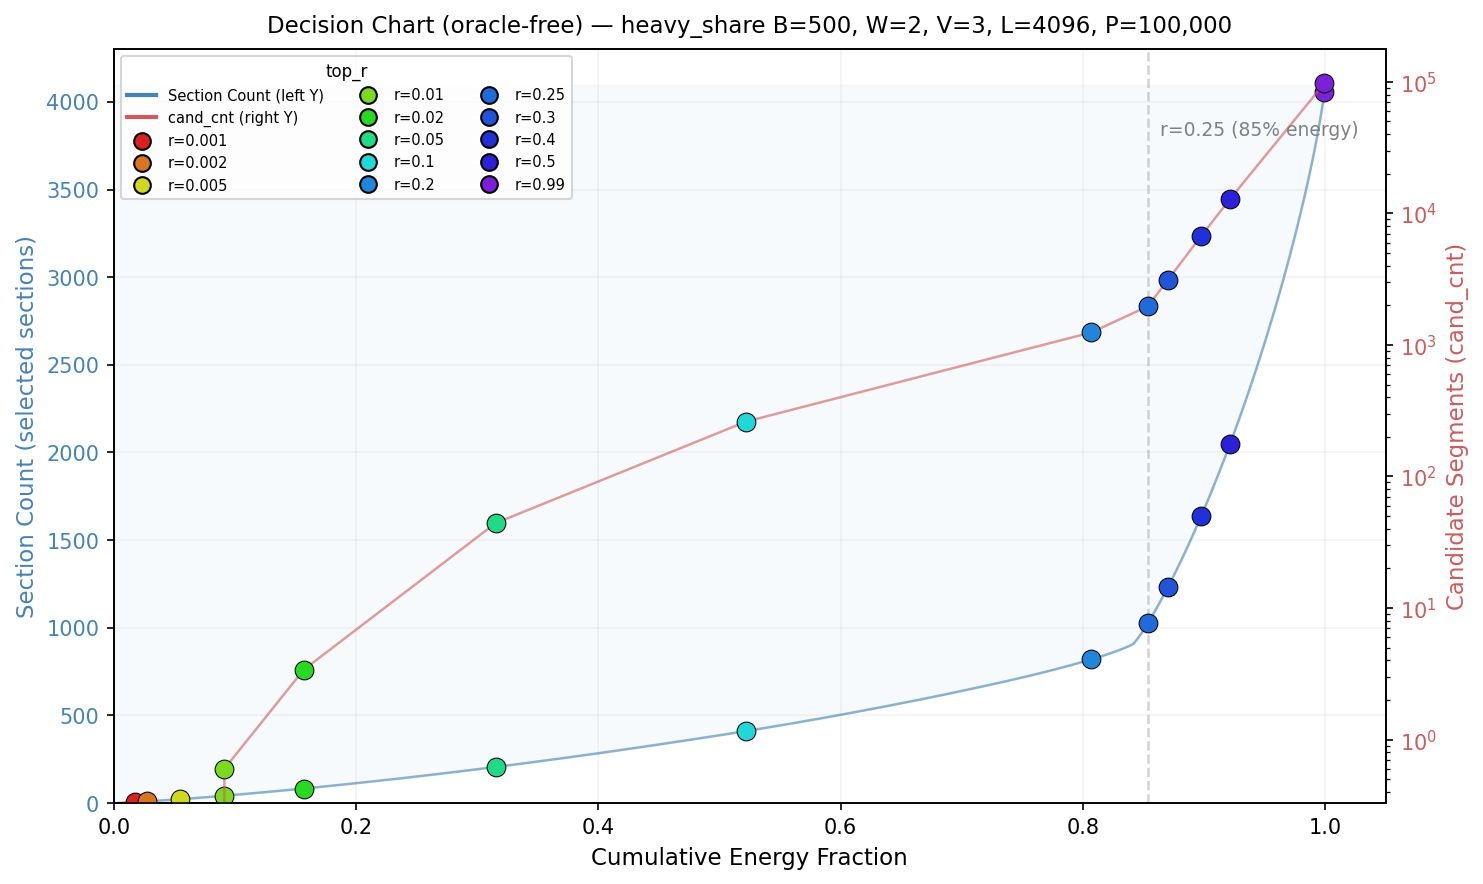
\includegraphics[width=\linewidth]{figures/decision_chart_energy_vs_cost.png}
\caption{Selected sections  (left axis) and candidate cost (right axis, log scale) plotted against cumulative energy fraction along the \texttt{top\_r} schedule. The two curves share a synchronized knee.}
\label{fig:c4-knee}
\end{figure}

Figure~\ref{fig:c4-knee} plots both quantities against cumulative energy fraction for a representative configuration. The first few top-ranked sections capture the bulk of the energy while candidate cost remains low; beyond a knee, additional sections contribute diminishing energy but candidate count accelerates sharply. This synchronized knee provides a natural stopping signal that requires no knowledge of the true~$B$: expansion halts when marginal energy gain per unit increase in candidate cost drops (implementation details in Supplement~\ref{sec:appendix-stoploss-details}). At the knee ($\mathrm{r_{top}}{=}0.25$), the cutoff captures approximately 85\% of total energy at a candidate fraction under~2\%. Doubling $\mathrm{r_{top}}$ beyond this point yields less than 5 percentage points of additional energy but increases candidate count by more than an order of magnitude.
Using ground-truth recall for offline verification, we find that this knee marks the point where additional candidate cost yields only modest recall gains (Supplement~Fig.~\ref{fig:c4-3-recall}).

\subsection{Same-Budget Comparison and Failure Regions}
\label{sec:eval-comparison}



Under a common sketch budget of approximately 512 KiB, we compare SCOUT, B2, and B3, focusing on the regimes in which triage and gating begin to fail.

\paragraph{Triage degrades under heavy-tail noise}

\begin{figure*}[!thbp]
\centering
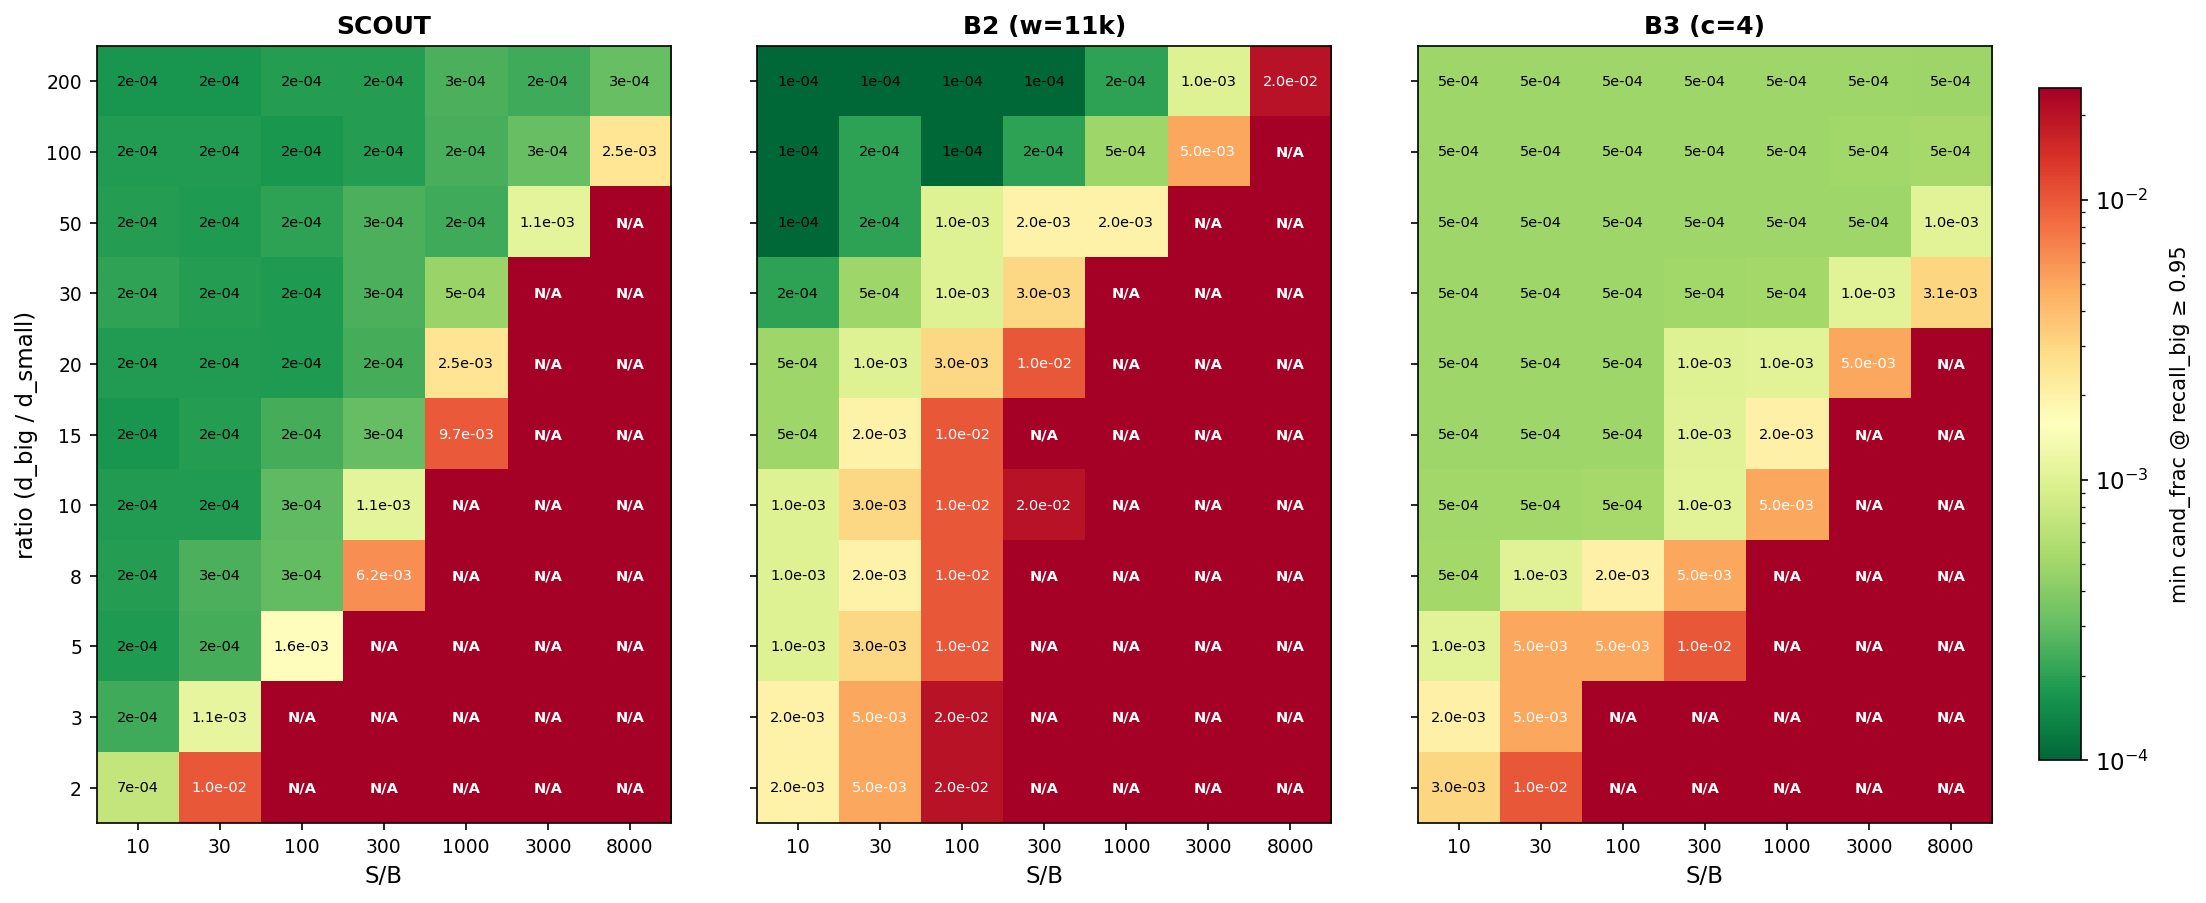
\includegraphics[width=0.9\linewidth]{figures/exp20v4_all_methods_heatmap_notitle.png}
\caption{Triage operating-point heatmap (same budget, single-round probe). Color encodes the minimum $\texttt{cand\_frac}$ achieving $\texttt{median(recall\_big)}\ge 0.95$ (log scale); N/A indicates the recall constraint cannot be met within the 2\% cap.}
\label{fig:c5-1}
\end{figure*}

We construct a family of mixed workloads with $P{=}100{,}000$ and $\texttt{total\_diff}{=}200{,}000$, comprising $B$ heavily dirty segments (each with $d_{\text{big}}$ diff keys) and $S$ noise segments (each with $d_{\text{small}}$ diff keys). The difficulty of separating heavy hitters from noise is parameterized along two axes: $\texttt{S/B}$ (noise-to-signal multiplier) and $\texttt{ratio}{=}d_{\text{big}}/d_{\text{small}}$ (separability). Figure~\ref{fig:c5-1} shows each method's feasible region on this two-dimensional parameter grid under a 2\% candidate budget cap. Greener cells indicate a lower required candidate fraction, whereas red cells marked as N/A denote configurations that cannot meet the recall constraint.

B2 degrades when heavy-tail noise collapses the per-segment ranking margin. With many noise segments (high $\texttt{S/B}$) and a small intensity gap (low $\texttt{ratio}$), mildly dirty segments flood the top-$K$ ranking and displace the genuinely heavy ones. At high separability ($\texttt{ratio}{=}200$), B2 achieves a slightly lower candidate fraction than SCOUT (${\sim}10^{-4}$ vs.\ ${\sim}2{\times}10^{-4}$), because direct ranking is highly effective when per-segment signals are already well separated; SCOUT pays a small halo cost from window aggregation. Once $\texttt{ratio}$ drops to single digits, however, B2 rapidly enters N/A. Doubling B2's memory to ${\sim}1$\,MiB does not change this picture: the low-separability region at $\texttt{ratio}\le 5$ remains unreachable (Supplement~\ref{sec:appendix-comp-triage}).

B3 is limited by the discrete granularity of its hierarchy. Once a leaf bucket is selected, the entire bucket must be expanded, so the candidate fraction increases in bucket-sized jumps rather than smoothly. Under heavy-tail noise, many buckets accumulate moderate discrepancy mass at the same time, which pushes the candidate set quickly toward the 2\% cap. An ablation over $B$ ($10{\to}100$) shows that SCOUT's feasible region shrinks by $25$\,pp, compared with $43$\,pp for B2 and $39$\,pp for B3. Additional checks, including doubling B2's memory, relaxing the candidate cap from 2\% to 5\% and 10\%, and sweeping $B$, do not change the qualitative comparison (Supplement~\ref{sec:appendix-comp-triage}).




\paragraph{Gating reliability under the same budget} \label{sec:eval-comp-gating}

\begin{figure}[!htbp]
\centering
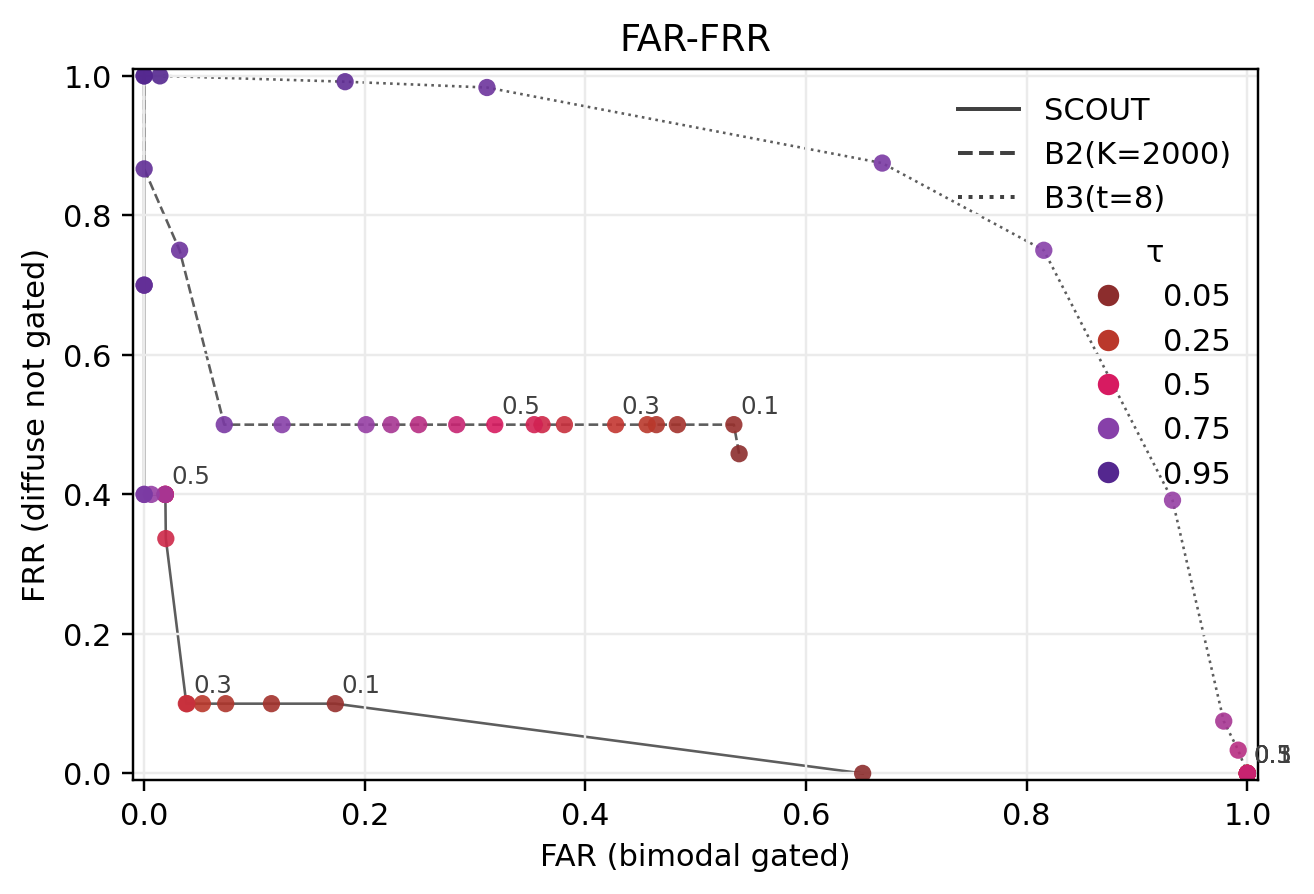
\includegraphics[width=0.92\linewidth]{figures/exp22v1_tradeoff_minT64_taulegend.png}
\caption{Conditional FAR--FRR trade-off (${\sim}512$\,KiB). Each point on a curve corresponds to a $\tau_{\text{gating}}$ threshold; the lower-left corner is the ideal region.}
\label{fig:c5-5-512}
\end{figure}

Figure~\ref{fig:c5-5-512} compares the conditional FAR--FRR trade-off of the three methods at ${\sim}512$\,KiB, treating \texttt{gate} as the positive class and conditioning on decisive (that is, non-\texttt{unknown}) samples. Full definitions, threshold sweeps, and supplementary analyses are provided in Supplement~\ref{sec:appendix-comp-gating}. SCOUT uses $K_{\text{eff}}/L$ as the gating statistic. B2 uses the fraction of total estimated mass not captured by its top-ranked segments, which stays near 0 when discrepancy mass is concentrated in a few segments and increases as the mass becomes more diffuse. B3 uses the maximum per-level fan-out ratio, using the most expanded level as a proxy for how diffusely the discrepancy spreads through the hierarchy.


\phantomsection\label{sec:eval-comp-far-frr}
Only SCOUT attains operating points with both low FAR and low FRR. Under the constraint $\texttt{FRR\_cond}\le 0.10$, $\tau_{\text{gating}}$ remains feasible across the interval $0.15$--$0.40$; at the representative point $\tau_{\text{gating}}{=}0.40$, $\texttt{FAR\_cond}\approx 0.038$ and $\texttt{FRR\_cond}{=}0.10$. The residual ${\sim}4\%$ conditional false-alarm rate is concentrated in borderline cases with high noise coverage. In contrast, B2's curve plateaus at $\texttt{FRR\_cond}{=}0.50$: regardless of threshold tuning, half of the diffuse samples are never intercepted, because heavy-tail noise dilutes concentrated faults to resemble diffuse ones, and B2's statistic cannot distinguish the two. B3 remains confined to the high-FAR, high-FRR region. Nearly all concentrated faults are misclassified as diffuse. Within shared buckets, collisions between dirty and clean segments inflate upper-level fan-out even for concentrated faults, leaving B3 with no usable trade-off interval (Supplement~\ref{sec:appendix-comp-gating}).

\subsection{Validation under YCSB-Driven Workloads}
\label{sec:eval-ycsb}

This section introduces segment-size skew as a robustness
dimension absent from the synthetic experiments above.
We use a YCSB Zipfian distribution ($\alpha{=}0.99$) to
generate the base keyspace and evaluate the following fault families:
\emph{Bimodal} (bounded-blast-radius concentrated faults),
\emph{Drift-shaped} (lag concentrated on hot segments),
and \emph{Uniform Diffuse} (broad low-rate anomalies).
Each family is instantiated at three data-scale tiers---Light
(20M records, $P{=}100{,}000$), Medium (200M), and Heavy
(2B)---which induce progressively denser segment fill states
under the same Zipfian workload.
A fourth family, \emph{Weighted Diffuse} (per-record loss
under segment-size skew), is further detailed in
Supplement~\ref{sec:appendix-ycsb-weighted} along with
parameterization details for all families
(Supplement Tables~\ref{tab:c6-trace-density}
and~\ref{tab:appendix-c6-faults}).

\paragraph{Gating}
The upper panel of Table~\ref{tab:c6-trace-triage} reports
SCOUT's $K_{\text{eff}}/L$, as \S\ref{sec:eval-comparison}
shows that neither baseline provides a reliable gating signal.
All four fault families form a clear gradient: Bimodal at
approximately $0.003$ (highly concentrated), Drift-shaped at
approximately $0.08$, Weighted Diffuse at approximately
$0.12$, and Uniform Diffuse at approximately $0.93$ (highly
diffuse). The wide separation between the first three
families ($K_{\text{eff}}/L \le 0.12$) and Uniform Diffuse
(${\ge}0.93$) leaves a broad margin for placing
$\tau_{\text{gating}}$: the first three families are admitted to the triage path while Uniform Diffuse is diverted to fallback.
$K_{\text{eff}}/L$ is nearly invariant across the three
data-scale tiers, indicating that the gating metric is
governed by segment-level fault shape rather than data
density. All families yield sufficient occupancy for decisive
gating across all three tiers, with no \texttt{unknown}
outcomes; full distributions are shown in
Supplement Figure~\ref{fig:c6-gating}.

\paragraph{Triage}
The lower panel of Table~\ref{tab:c6-trace-triage} reports the
minimum candidate fraction achieving
$\texttt{recall\_big}\ge 0.95$ under a 2\% cap. Bimodal faults
yield a stable candidate fraction of $3{\times}10^{-5}$;
Drift-shaped faults yield approximately
$7.3{\times}10^{-4}$. Across the three tiers, candidate
fractions change little: with $P$ and the segment-level fault
pattern held fixed, increasing the record count mainly
densifies segment fill rather than changing the sketch-level
concentration pattern. Uniform Diffuse does not appear in the
triage panel because gating diverts it to fallback.

\paragraph{Sizing}
Drift-shaped faults are the hardest sizing case because they
combine segment-size skew with concentration on hot segments.
With the Bessel correction applied, the de-drifted estimator
achieves a median relative error of 0.8\%--1.4\% across
the three tiers (p90 $\le 2.8\%$), matching the accuracy
observed under the uniform settings of
\S\ref{sec:eval-dedrift}; raw-control results are reported in
Supplement Table~\ref{tab:c6-sizing}.

\begin{table}[!thbp]
\caption{YCSB-driven validation summary across data-scale tiers.
Upper: gating statistic; lower: triage candidate fraction.}
\label{tab:c6-trace-triage}
\centering
\small
\setlength{\tabcolsep}{3pt}
\begin{tabular}{lccc}
\toprule
Family & Light & Medium & Heavy \\
\midrule
\multicolumn{4}{c}{SCOUT Gating: median $K_{\text{eff}}/L$} \\
\midrule
Bimodal          & 0.003 & 0.003 & 0.003 \\
Drift-shaped     & 0.082 & 0.082 & 0.081 \\
Weighted Diffuse & 0.122 & 0.118 & 0.120 \\
Uniform Diffuse  & 0.931 & 0.938 & 0.939 \\
\midrule
\multicolumn{4}{c}{SCOUT Triage: min $\texttt{cand\_frac}$
  at $\texttt{recall\_big}{\ge}0.95$} \\
\midrule
Bimodal      & $3{\times}10^{-5}$ & $3{\times}10^{-5}$ & $3{\times}10^{-5}$ \\
Drift-shaped & $7.3{\times}10^{-4}$ & $7.4{\times}10^{-4}$ & $7.3{\times}10^{-4}$ \\
\bottomrule
\end{tabular}
\end{table}

Sections~\ref{sec:eval-spatial}--\ref{sec:eval-ycsb} evaluate SCOUT's triage, sizing, and gating behavior across controlled synthetic workloads and YCSB-driven skewed workloads. Because
these results assume uniform hashing at the probe interface, we additionally verify in Supplement~\ref{sec:appendix-hash} that the triage operating points remain stable across three hash
implementations, two key structures, and $k\in\{1,2,3\}$.
\phantomsection\label{sec:eval-summary}

\section{Discussion}
\label{sec:discussion}

SCOUT is designed for deployments where reconciliation runs as
a continuous background function, most rounds are expected to
be clean, and exact verification is expensive relative to a
fixed-size probe exchange. In this setting, the three probe
outputs serve distinct operational roles: sizing always
provides a severity signal; gating decides whether the current
discrepancy shape supports economical candidate
compression; and triage narrows the verification scope when
the discrepancy is sufficiently concentrated. Table~\ref{tab:probe-outcome-mapping}
summarizes the round-level interpretation. In the common
clean-round case, reconciliation terminates after a single
fixed-cost probe exchange, without invoking downstream
verification. Precise localization and repair within the
candidate scope remain delegated to downstream mechanisms such
as Merkle trees or IBLTs; SCOUT's role ends at diagnosis.


\begin{table}[!htbp]
\caption{Representative operational scenarios and typical probe outcomes.}
\label{tab:probe-outcome-mapping}
\centering
\footnotesize
\setlength{\tabcolsep}{0.2pt}
\begin{tabular}{@{}p{0.26\linewidth}p{0.15\linewidth}p{0.15\linewidth}p{0.45\linewidth}@{}}
\toprule
Scenario & $\hat{D}$ & $g$ & Action \\
\midrule
Normal round
  & $\approx 0$ 
  & -- 
  & {skip downstream verification} \\[2pt]

\shortstack[l]{Shard failure} 
  & varies 
  & \texttt{notgate} 
  & \shortstack[l]{triage, then verify on $\mathcal{C}$} \\[2pt]

\shortstack[l]{One-sided\\backlog}
  & large
  & varies
  & \shortstack[l]{severity alert; triage if\\shape admits, else fallback} \\[2pt]


\shortstack[l]{Diffuse dis-\\crepancy} 
  & \shortstack[l]{moderate\\or large} 
  & \texttt{gate} 
  & \shortstack[l]{bypass triage; use fallback} \\[2pt]

\shortstack[l]{Low obser-\\vability} 
  & varies 
  & \texttt{unknown} 
  & \shortstack[l]{defer, capped triage, or fallback} \\[2pt]

\shortstack[l]{Segmenter\\misconfiguration}
  & $\approx$ total 
  & \texttt{--} 
  & \shortstack[l]{inspect config} \\
\bottomrule
\end{tabular}
\end{table}


Among the probe outcomes in Table~\ref{tab:probe-outcome-mapping}, \texttt{unknown} merits separate discussion. It is an explicit abstention:
  the probe lacks sufficient statistical support for a reliable shape judgment. The most common trigger is a small number of concurrent
faults, which leaves too few sections energized for $K_{\mathrm{eff}}/L$ to reliably separate concentrated from diffuse patterns.
Paradoxically, this is also the regime where triage is most effective, since a small $B$ yields high signal separability and strong candidate
  compression. In deployment, \texttt{unknown} rounds can still be acted upon by combining $\hat{D}$ with other observables such as occupancy:
  deferring when $\hat{D}$ is small, or proceeding with a capped triage pass when $\hat{D}$ is large. What SCOUT withholds is a shape-based
recommendation, not the scale signal itself.

A natural question is whether the discrepancy axes used
in our evaluation---concentration, diffuseness, and side
imbalance---provide a useful abstraction for fault scenarios
encountered in practice. Our results suggest that they capture
several common manifestations relevant to continuous
reconciliation: concentrated discrepancies tend to benefit
from triage, diffuse ones are more likely to be diverted by
gating, and asymmetric ones still admit a stable sizing signal
through de-drifted energy. This abstraction is not intended as
an exhaustive fault taxonomy. One scenario that may appear to
fall outside it is spatially correlated dirty segments in the
underlying key space; however, after hash-based segment
mapping, such correlation often appears as a larger effective
$B$, which is already reflected in the capacity-degradation
dimension characterized in \S\ref{sec:eval-operating}.


Two limitations remain. First, the synthetic and YCSB-driven
workloads do not establish how frequently each discrepancy
class arises in production, nor whether additional classes
emerge under real operational correlations or temporal
patterns. Second, under extreme multi-fault overlap
($B \cdot W$ approaching~$L$), the sparse-overlap
approximation used in the candidate-size analysis begins to
break down, and this regime would benefit from a tighter
characterization.

\section{Conclusion}
\label{sec:conclusion}

SCOUT is a single-round, fixed-budget diagnostic probe that
serves as a front-end to precise downstream verification in
heterogeneous replication. From one sketch exchange, it
jointly provides discrepancy sizing, shape-based gating, and
candidate-scope triage, all derived from a shared
de-drifted statistical substrate. Across synthetic stress
tests, same-budget baseline comparisons, and YCSB-driven
workloads, the results show that these three outputs can be
combined within a single fixed-budget probe while remaining
useful across concentrated, diffuse, and asymmetric
discrepancy regimes.

More broadly, SCOUT shows that continuous reconciliation need
not pay full validation cost on every round. By separating
diagnosis from exact repair, clean rounds terminate after a
fixed probe exchange, while anomalous rounds invoke more
expensive downstream verification only when the observed
discrepancy warrants it. An important next step is to
validate how the discrepancy classes studied here are
distributed in production traces and deployments.


\bibliographystyle{unsrt}
\bibliography{ref}
\end{document}



